\section*{Supplementary material}

\subsection{Correlation between divergences that share branches}\label{sec:share}

Landscapes of divergence can be correlated by their definition, as they can share part of their histories.
In most of our analyses (except for \lcref{fig:land_cors_bo}), we do not show the correlations for such cases but below we describe how this sharing would affect correlations (using a simplified theory).
For example, in \lcref{fig:conceptual_tree} $d_{VX}$ and $d_{XY}$ share the branch $X$;
depending on how the length of the branch $X$ compares to the total tree length, these two landscapes are bound to be correlated.
Assuming that mutations follow a Poisson process and that coalescences happen instantaneously, we derive the following.
There are three non-overlapping parts in the tree between these, the branch from the $XY$ ancestor to $X$ with length $\E [\tau_X]=T_{XY}$, the branch from the $XY$ ancestor to $Y$ with length $\E [\tau_Y]=T_{XY}$ and the branch from $V$ to the $XY$ ancestor with length $\E[\tau_V]=2T_{VWXY} - T_{XY}$.
If we just consider the genealogical definition of divergence and assume $d_{VX} = \tau_V + \tau_X$ and $d_{XY} = \tau_X + \tau_Y$ (\ie, ignoring the contributions of ancestral diversity to divergence), then

\begin{align*}
\Cov [ d_{VX}, d_{XY} ] &= \Cov [ \tau_X + \tau_V, \tau_X + \tau_Y ] \\
 &= \Cov [ \tau_X, \tau_X ] + \cancelto{0}{\Cov [ \tau_X, \tau_Y ]} + \cancelto{0}{\Cov [ \tau_V, \tau_X ]} + \cancelto{0}{\Cov [ \tau_V, \tau_Y ]} \\
 &= \Var(\tau_X) = \E[\tau_X] = T_X
\end{align*}

Therefore, 

\begin{align*}
\Cor [ d_{VX}, d_{XY} ] &= \frac{\Cov [ \tau_X + \tau_V, \tau_X + \tau_Y ]}{\sqrt{\Var[\tau_X + \tau_V]\Var[\tau_X + \tau_Y]}} \\
 &= \sqrt{\frac{\Var[\tau_X]^2}{(\Var[\tau_X]+\Var[\tau_V])(\Var[\tau_X]+\Var[\tau_Y])}} \\
 &= \sqrt{\frac{\Var[\tau_X]}{\Var[\tau_X]+\Var[\tau_V]}\frac{\Var[\tau_X]}{\Var[\tau_X]+\Var[\tau_Y]}} \\ 
 &= \sqrt{\frac{T_X}{T_X+T_V}\frac{T_X}{T_X +T_Y}} \\
 &= \sqrt{p_{d_{VX}} p_{d_{XY}}}
\end{align*}

where $p_{d_{VX}} = \frac{T_X}{T_X+T_V}$ is the proportion of $d_{VX}$ that is shared with $d_{XY}$, and $p_{d_{XY}} = \frac{T_X}{T_X+T_Y}$ is the proportion of $d_{XY}$ that is shared with $d_{VX}$.


% latex table generated in R 3.6.3 by xtable 1.8-4 package
% Wed Jan 25 14:17:28 2023
\begin{table}
\tiny
\centering
\begin{tabular}{rrrrll}
  \hline
$\mu_N$ & $\mu_P$ & $\bar{s}_N$ & $\bar{s}_P$ & Regime & $\mu_{SD}$ \\ 
  \hline
$0$ & $0$ & $0$ & $0$ & Neutral & 0 \\ 
  $0$ & $0$ & $0$ & $0$ & Variable $\mu$ & 0.005 \\ 
  $0$ & $0$ & $0$ & $0$ & Variable $\mu$ & 0.007 \\ 
  $0$ & $0$ & $0$ & $0$ & Variable $\mu$ & 0.011 \\ 
  $0$ & $0$ & $0$ & $0$ & Variable $\mu$ & 0.016 \\ 
  $0$ & $0$ & $0$ & $0$ & Variable $\mu$ & 0.023 \\ 
  $0$ & $0$ & $0$ & $0$ & Variable $\mu$ & 0.033 \\ 
  $0$ & $0$ & $0$ & $0$ & Variable $\mu$ & 0.048 \\ 
  $0$ & $0$ & $0$ & $0$ & Variable $\mu$ & 0.070 \\ 
  $0$ & $0$ & $0$ & $0$ & Variable $\mu$ & 0.103 \\ 
  $0$ & $0$ & $0$ & $0$ & Variable $\mu$ & 0.150 \\ 
  $0$ & $1 \times 10^{-12}$ & $0$ & $1 \times 10^{-2}$ & Beneficial & 0 \\ 
  $0$ & $1 \times 10^{-11}$ & $0$ & $1 \times 10^{-2}$ & Beneficial & 0 \\ 
  $2 \times 10^{-9}$ & $0$ & $-3 \times 10^{-2}$ & $0$ & Deleterious & 0 \\ 
  $2 \times 10^{-9}$ & $1 \times 10^{-11}$ & $-3 \times 10^{-2}$ & $1 \times 10^{-2}$ & Both & 0 \\ 
  $2 \times 10^{-9}$ & $0$ & $-1.5 \times 10^{-2}$ & $0$ & Deleterious & 0 \\ 
  $2 \times 10^{-9}$ & $1 \times 10^{-11}$ & $-1.5 \times 10^{-2}$ & $1 \times 10^{-2}$ & Both & 0 \\ 
  $2 \times 10^{-9}$ & $0$ & $-1 \times 10^{-2}$ & $0$ & Deleterious & 0 \\ 
  $2 \times 10^{-9}$ & $1 \times 10^{-12}$ & $-1 \times 10^{-2}$ & $5 \times 10^{-3}$ & Both & 0 \\ 
  $2 \times 10^{-9}$ & $1 \times 10^{-12}$ & $-1 \times 10^{-2}$ & $1 \times 10^{-2}$ & Both & 0 \\ 
  $2 \times 10^{-9}$ & $0$ & $-3 \times 10^{-3}$ & $0$ & Deleterious & 0 \\ 
  $2 \times 10^{-9}$ & $1 \times 10^{-12}$ & $-3 \times 10^{-3}$ & $5 \times 10^{-3}$ & Both & 0 \\ 
  $2 \times 10^{-9}$ & $1 \times 10^{-12}$ & $-3 \times 10^{-3}$ & $1 \times 10^{-2}$ & Both & 0 \\ 
  $2 \times 10^{-9}$ & $0$ & $-1 \times 10^{-3}$ & $0$ & Deleterious & 0 \\ 
  $2 \times 10^{-9}$ & $1 \times 10^{-11}$ & $-1 \times 10^{-3}$ & $1 \times 10^{-2}$ & Both & 0 \\ 
  $6 \times 10^{-9}$ & $0$ & $-3 \times 10^{-2}$ & $0$ & Deleterious & 0 \\ 
  $6 \times 10^{-9}$ & $1 \times 10^{-11}$ & $-3 \times 10^{-2}$ & $1 \times 10^{-2}$ & Both & 0 \\ 
  $6 \times 10^{-9}$ & $0$ & $-1.5 \times 10^{-2}$ & $0$ & Deleterious & 0 \\ 
  $6 \times 10^{-9}$ & $1 \times 10^{-11}$ & $-1.5 \times 10^{-2}$ & $1 \times 10^{-2}$ & Both & 0 \\ 
  $1 \times 10^{-8}$ & $1 \times 10^{-11}$ & $-1 \times 10^{-3}$ & $1 \times 10^{-2}$ & Both & 0 \\ 
  $1.2 \times 10^{-8}$ & $0$ & $-3 \times 10^{-2}$ & $0$ & Deleterious & 0 \\ 
  $1.2 \times 10^{-8}$ & $1 \times 10^{-12}$ & $-3 \times 10^{-2}$ & $1 \times 10^{-2}$ & Both & 0 \\ 
  $1.2 \times 10^{-8}$ & $1 \times 10^{-12}$ & $-3 \times 10^{-2}$ & $1 \times 10^{-2}$ & Both & 0.005 \\ 
  $1.2 \times 10^{-8}$ & $1 \times 10^{-12}$ & $-3 \times 10^{-2}$ & $1 \times 10^{-2}$ & Both & 0.007 \\ 
  $1.2 \times 10^{-8}$ & $1 \times 10^{-12}$ & $-3 \times 10^{-2}$ & $1 \times 10^{-2}$ & Both & 0.011 \\ 
  $1.2 \times 10^{-8}$ & $1 \times 10^{-12}$ & $-3 \times 10^{-2}$ & $1 \times 10^{-2}$ & Both & 0.016 \\ 
  $1.2 \times 10^{-8}$ & $1 \times 10^{-12}$ & $-3 \times 10^{-2}$ & $1 \times 10^{-2}$ & Both & 0.023 \\ 
  $1.2 \times 10^{-8}$ & $1 \times 10^{-12}$ & $-3 \times 10^{-2}$ & $1 \times 10^{-2}$ & Both & 0.033 \\ 
  $1.2 \times 10^{-8}$ & $1 \times 10^{-12}$ & $-3 \times 10^{-2}$ & $1 \times 10^{-2}$ & Both & 0.048 \\ 
  $1.2 \times 10^{-8}$ & $1 \times 10^{-12}$ & $-3 \times 10^{-2}$ & $1 \times 10^{-2}$ & Both & 0.070 \\ 
  $1.2 \times 10^{-8}$ & $1 \times 10^{-12}$ & $-3 \times 10^{-2}$ & $1 \times 10^{-2}$ & Both & 0.103 \\ 
  $1.2 \times 10^{-8}$ & $1 \times 10^{-12}$ & $-3 \times 10^{-2}$ & $1 \times 10^{-2}$ & Both & 0.150 \\ 
  $1.2 \times 10^{-8}$ & $1 \times 10^{-11}$ & $-3 \times 10^{-2}$ & $1 \times 10^{-2}$ & Both & 0 \\ 
  $1.4 \times 10^{-8}$ & $0$ & $-3 \times 10^{-2}$ & $0$ & Deleterious & 0 \\ 
  $1.4 \times 10^{-8}$ & $0$ & $-3 \times 10^{-2}$ & $0$ & Deleterious & 0.005 \\ 
  $1.4 \times 10^{-8}$ & $0$ & $-3 \times 10^{-2}$ & $0$ & Deleterious & 0.007 \\ 
  $1.4 \times 10^{-8}$ & $0$ & $-3 \times 10^{-2}$ & $0$ & Deleterious & 0.011 \\ 
  $1.4 \times 10^{-8}$ & $0$ & $-3 \times 10^{-2}$ & $0$ & Deleterious & 0.016 \\ 
  $1.4 \times 10^{-8}$ & $0$ & $-3 \times 10^{-2}$ & $0$ & Deleterious & 0.023 \\ 
  $1.4 \times 10^{-8}$ & $0$ & $-3 \times 10^{-2}$ & $0$ & Deleterious & 0.033 \\ 
  $1.4 \times 10^{-8}$ & $0$ & $-3 \times 10^{-2}$ & $0$ & Deleterious & 0.048 \\ 
  $1.4 \times 10^{-8}$ & $0$ & $-3 \times 10^{-2}$ & $0$ & Deleterious & 0.070 \\ 
  $1.4 \times 10^{-8}$ & $0$ & $-3 \times 10^{-2}$ & $0$ & Deleterious & 0.103 \\ 
  $1.4 \times 10^{-8}$ & $0$ & $-3 \times 10^{-2}$ & $0$ & Deleterious & 0.150 \\ 
  $1.4 \times 10^{-8}$ & $1 \times 10^{-12}$ & $-3 \times 10^{-2}$ & $1 \times 10^{-2}$ & Both & 0 \\ 
  $1.4 \times 10^{-8}$ & $1 \times 10^{-11}$ & $-3 \times 10^{-2}$ & $1 \times 10^{-2}$ & Both & 0 \\ 
   \hline
\end{tabular}
\label{tab:sim_params}
\caption{Parameter space explored with simulations. $\mu_N$ and $\mu_P$ are the rates of mutations under negative and positive selection, respectively.
$\bar{s}_N$ and $\bar{s}_P$ and the mean fitness effects of negatively and positively selected mutations. $\mu_{SD}$ is the scaled standard deviation of the mutation rate map. See \autoref{tab:sim_space} and \autoref{sec:methods:simu} for more details.} 
\end{table}


\begin{figure}[htp]
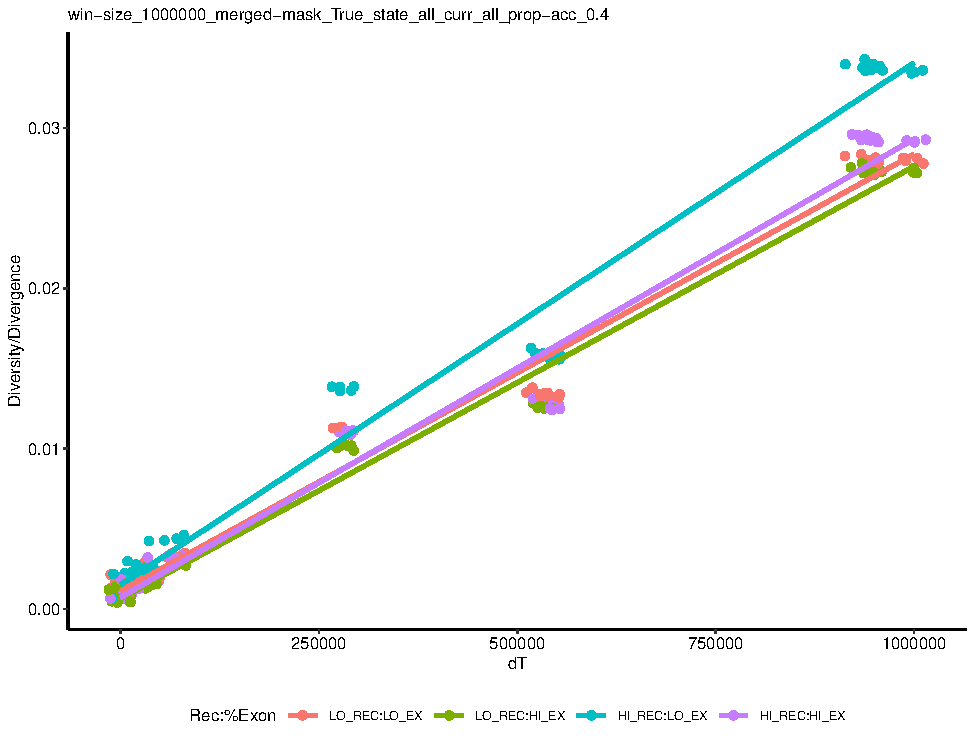
\includegraphics[width=\linewidth]{{figures/chr12-pidxy-change-dT.pdf}}
\centering
\caption{
Effect of exon density and recombination rate on the accumulation of genetic divergence in chromosome 12 with phylogenetic distance.
Within-species genetic diversities are shown at $dT=0$.
Mean diversity and divergences were computed for four groups depending on whether they fell or not on the top $90\%$ percentile of recombination rate and exon density.
}
\label{fig:pidxy-change}
\end{figure}

\begin{figure}[htp]
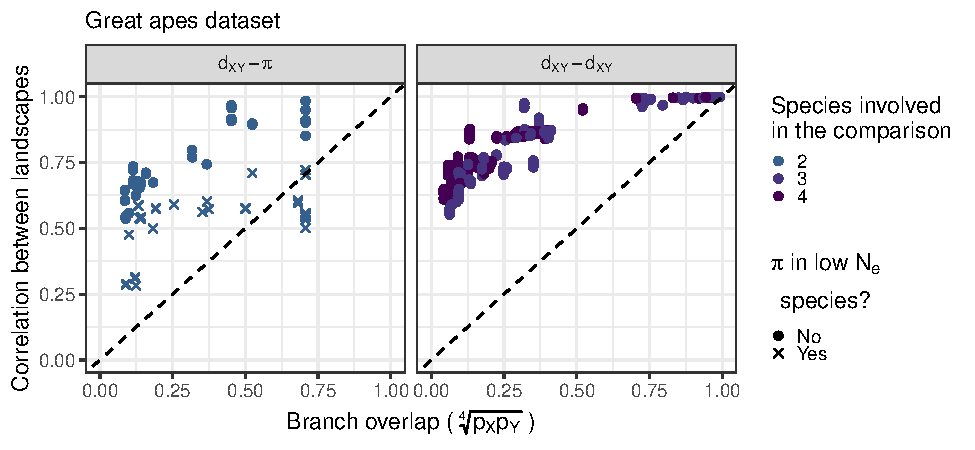
\includegraphics[width=\linewidth]{{figures/cor-pidxy-branchoverlap_data.pdf}}
\centering
\caption{
Correlations between landscapes of diversity and divergence for comparisons with branch overlap.
For example, diversity in humans and divergence between humans and bonobos share part of their history.
Each point on the plots correspond to the (Spearman) correlation between two landscapes of diversity/divergence, computed on 1Mb windows across the entire genome. 
Correlations were split by type of landscapes compared ($\pi-d_{XY}$, $d_{XY}-d_{XY}$). 
The x-axis is a metric of expected branch overlap between the landscapes. See \autoref{sec:share} for more information.
Note that species with low $N_e$ (bonobos, eastern gorillas and western chimps) have a different point shape. 
The colors reflect the number of species involved in the comparison.
For example, the comparison between human-western gorilla and eastern chimp-Sumatran orangutan divergences includes four different species.
On the other hand, the comparison between  human-western gorilla and human-Sumatran orangutan divergences includes just three species.
}
\label{fig:land_cors_bo}
\end{figure}

\begin{landscape}
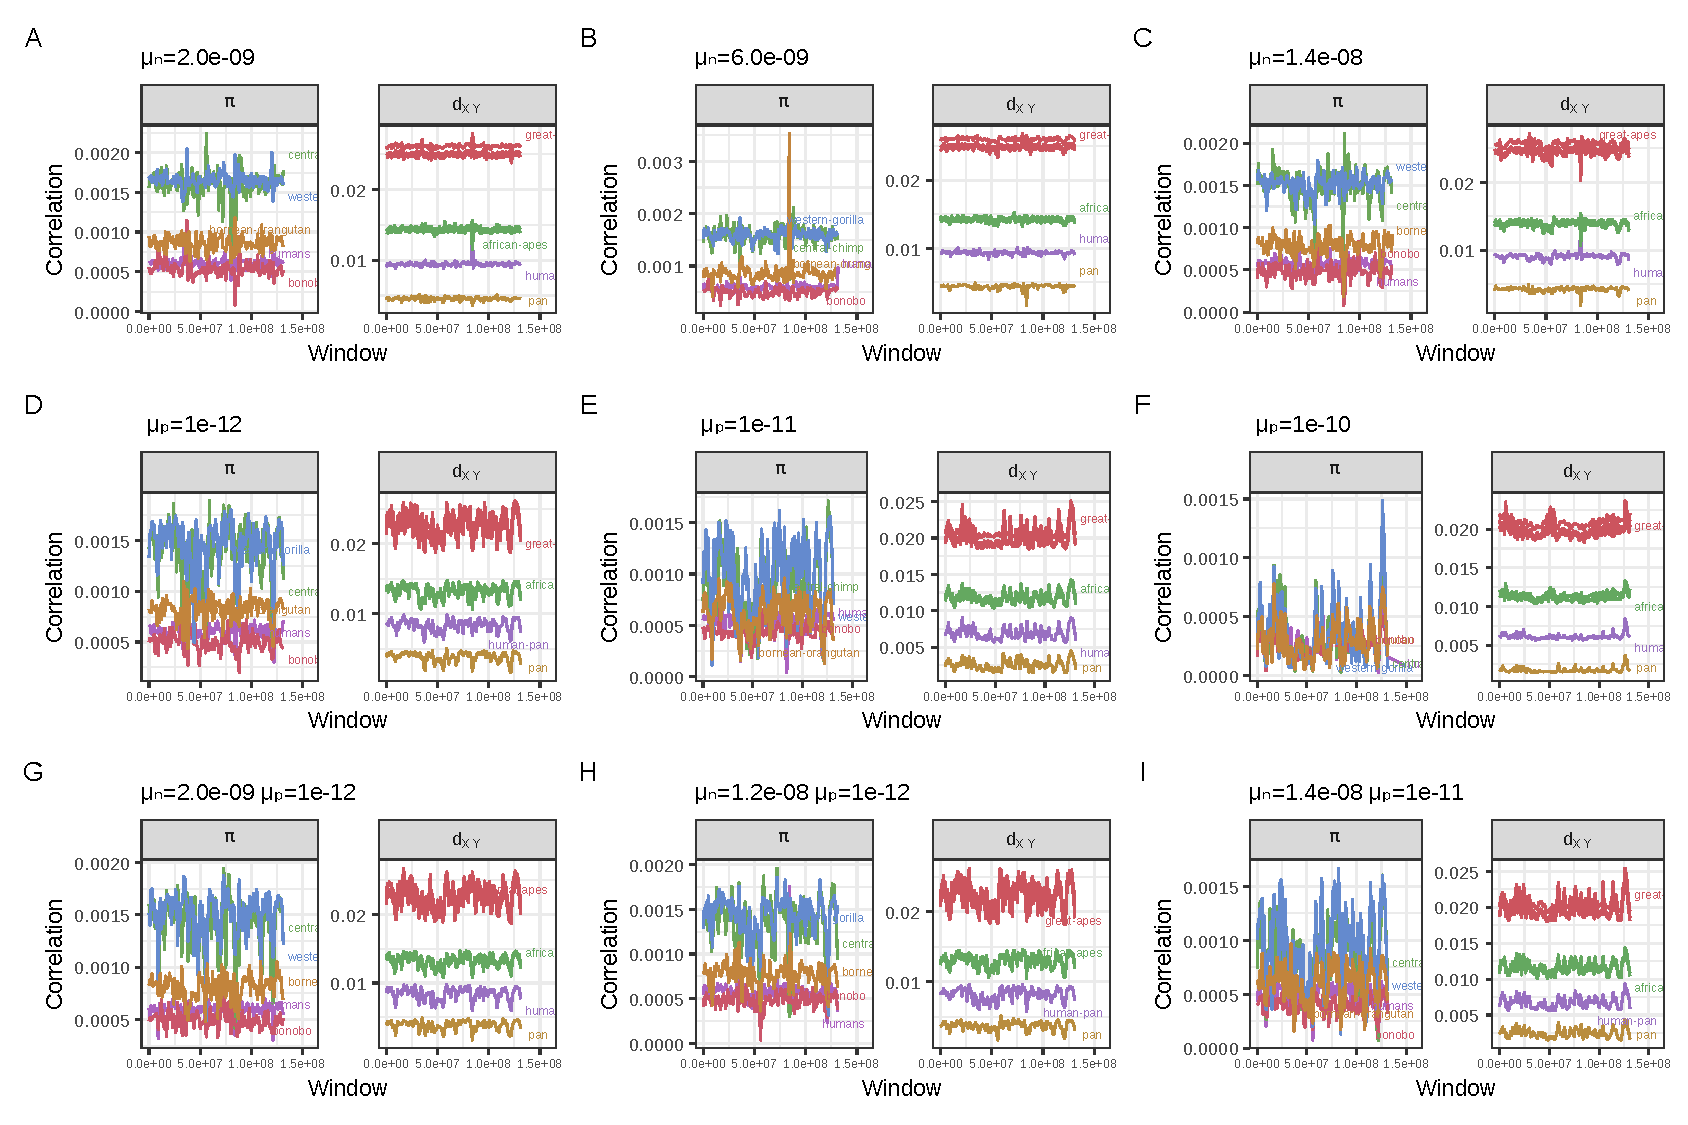
\includepdf[pages=1,scale=0.8,landscape, pagecommand={
\null\enlargethispage{3\baselineskip}\vfill
\thispagestyle{pdflandscape}
\captionof{figure}{
Landscapes of diversity and divergence in selected simulations with natural selection.
The selection parameters $\mu_n$ and $\mu_p$ are the rate of mutations in exons with negative and positive fitness effects, respectively.
The mean fitness effect was $\bar{s}=-0.03$ for deleterious mutations and $\bar{s}=0.01$ for beneficial mutations (see \autoref{sec:methods:simu} for more details).
Other details are as in \lcref{fig:chr12_landscapes}.
}
}]{figures/chr12-landscapes_selected-sel-sims.pdf}
%\fillandplacepagenumber
\end{landscape}

\begin{figure}[htp]
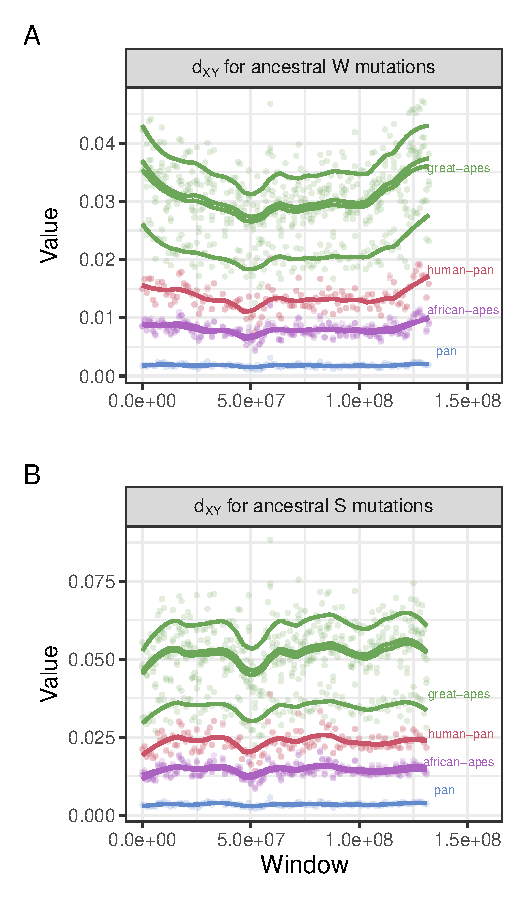
\includegraphics[]{{figures/anc-partitioned_dxy_landscapes_data.pdf}}
\centering
\caption{
Landscapes of divergence partitioned by allele state in the ancestor.
Ancestral states were assumed to be the same as seen in rhesus macaques (RheMac2),
and sites not called in macaques were not used.
$d_{XY}$ for W sites is simply the mean pairwise differences between samples in species $X$ and $Y$ per ancestral W sites (A/T).
Similar reasoning applies for $d_{XY}$ for S ancestral sites, but only considering (G/C) sites.
Points were colored by the most common recent ancestor of the two species compared in each divergence.
Lines were fitted using local linear regression.
Note that for ancestrally weak mutations (A) there is an increase in divergence at the ends of the chromosomes,
but that is not seen for ancestrally strong mutations (B).
}
\label{fig:anc-partitioned_dxy}
\end{figure}

\begin{figure}[htp]
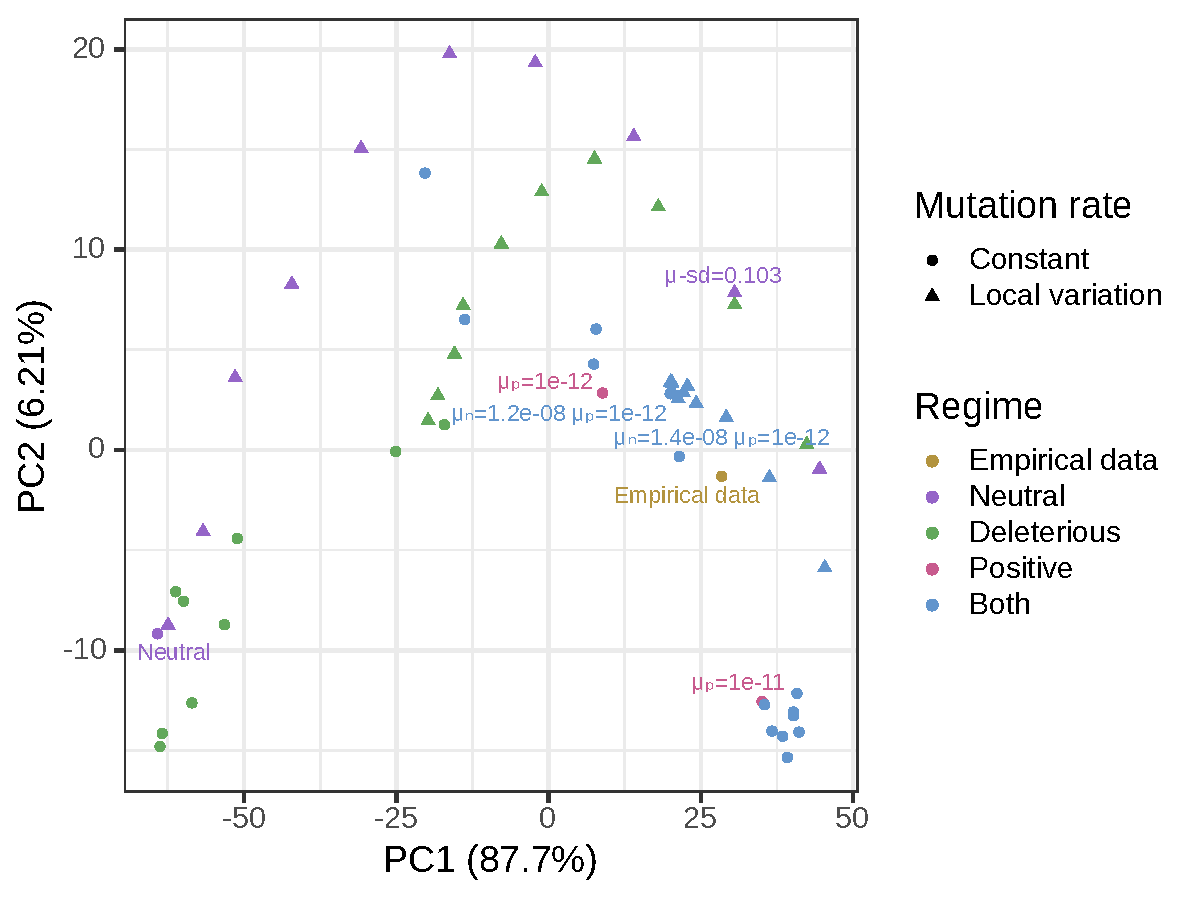
\includegraphics[width=0.7\linewidth]{{figures/data-and-sims_pca_500kb.pdf}}
\centering
\caption[PCA visualization of data and simulations at 500Kb scale]{
PCA visualization of data and simulations at 500Kb.
The colors differentiate the empirical data from simulations with different parameters:
Neutral refers to the simulation without any selection,
Deleterious refers to simulations with deleterious mutations,
Positive refers to simulations with beneficial mutations,
Both refers to simulations with both beneficial and deleterious mutations.
The shape of the points differentiate simulations with constant mutation rate along the genome and variable local mutation rates.
Principal component analysis (PCA) applied to a matrix with all pairwise correlations between landscapes across the great apes 
(including $\pi-\pi$, $\pi-d_{XY}$ and $d_{XY}-d_{XY}$ comparisons) for the great apes dataset and simulations (with selection and with mutation rate variation).
We excluded simulations with $\mu_p \geq \expnumber{1}{-10}$ from the PCA analysis because PC2 was capturing negative correlations caused by strong positive selection --- as seen in \lcref{fig:sims_land_cors}[F].
}
\label{fig:pca500kb}
\end{figure}

\begin{figure}[htp]
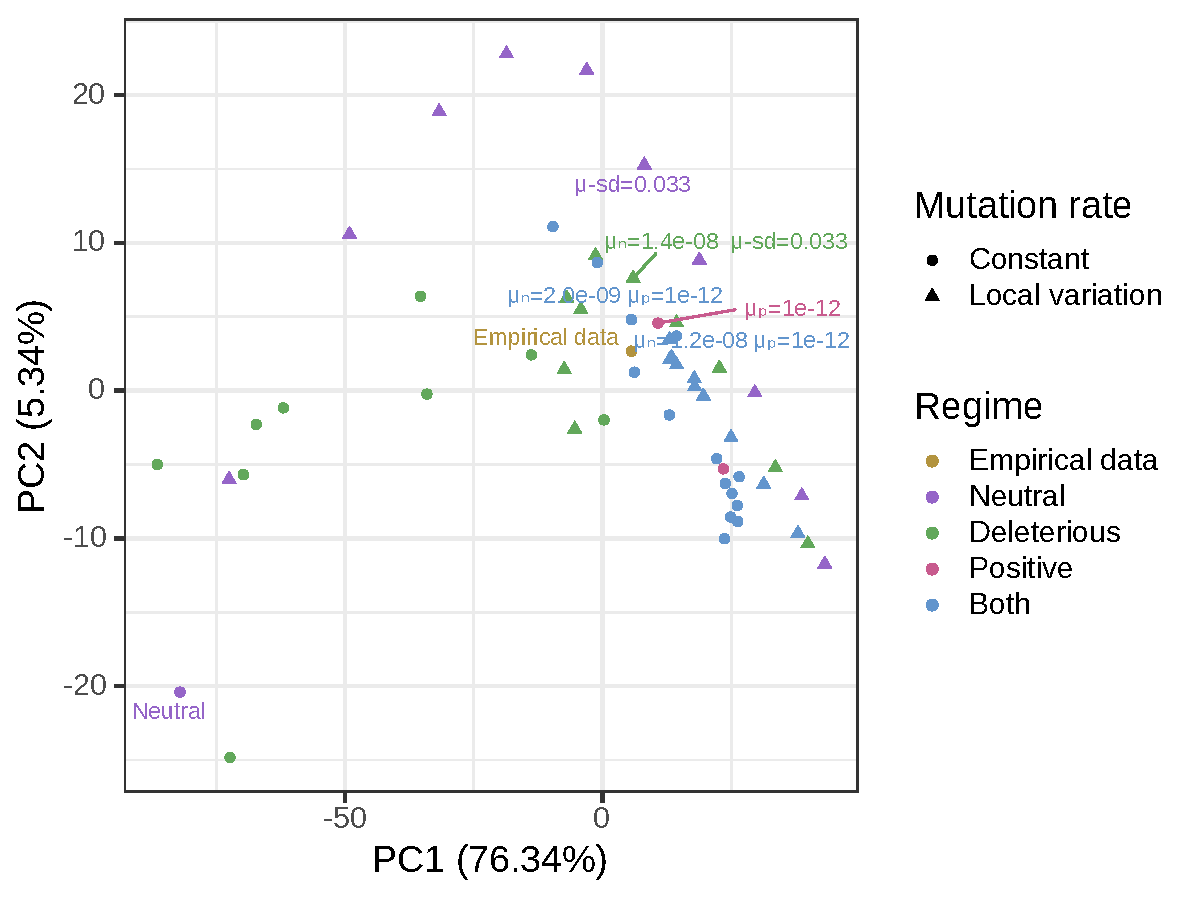
\includegraphics[width=0.7\linewidth]{{figures/data-and-sims_pca_5mb.pdf}}
\centering
\caption[PCA visualization of data and simulations at 5Mb scale]{
PCA visualization of data and simulations at 5Mb.
The colors differentiate the empirical data from simulations with different parameters:
Neutral refers to the simulation without any selection,
Deleterious refers to simulations with deleterious mutations,
Positive refers to simulations with beneficial mutations,
Both refers to simulations with both beneficial and deleterious mutations.
The shape of the points differentiate simulations with constant mutation rate along the genome and variable local mutation rates.
Principal component analysis (PCA) applied to a matrix with all pairwise correlations between landscapes across the great apes 
(including $\pi-\pi$, $\pi-d_{XY}$ and $d_{XY}-d_{XY}$ comparisons) for the great apes dataset and simulations (with selection and with mutation rate variation).
We excluded simulations with $\mu_p \geq \expnumber{1}{-10}$ from the PCA analysis because PC2 was capturing negative correlations caused by strong positive selection --- as seen in \lcref{fig:sims_land_cors}[F].
}
\label{fig:pca5mb}
\end{figure}

\begin{figure}[htp]
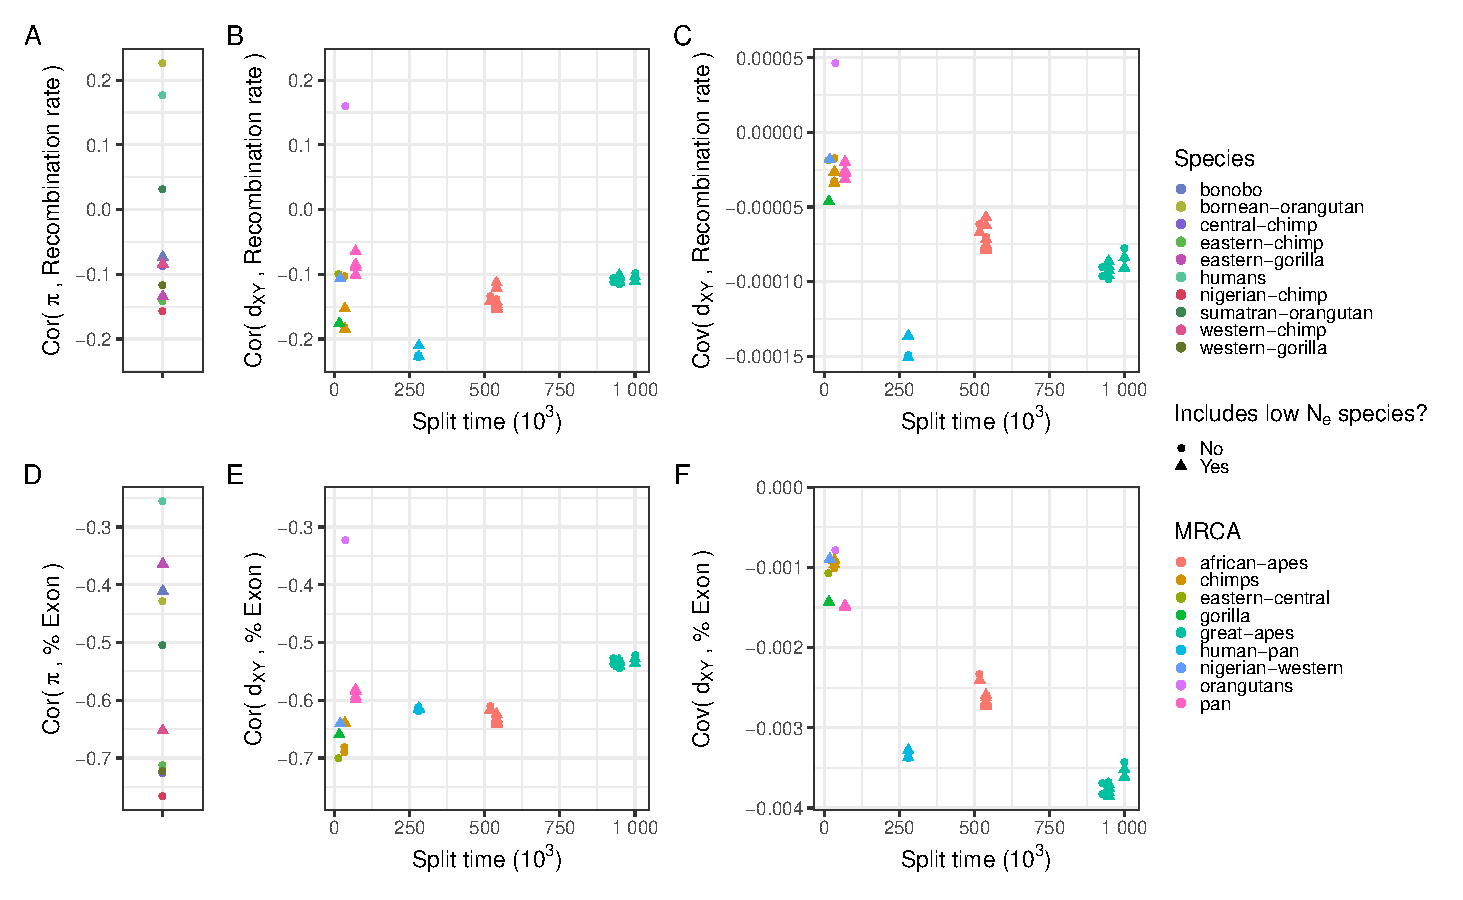
\includegraphics[width=\linewidth]{{figures/cor-pidxy-annot-central_data.pdf}}
\centering
\caption{
Correlations and covariances between landscapes of diversity and divergence and annotation features in the real great apes data.
Only windows in the middle half of chromosome 12 were included.
Compare to \lcref{fig:annot_cors}.
}
\label{fig:annot_cors_center}
\end{figure}

\begin{figure}[htp]
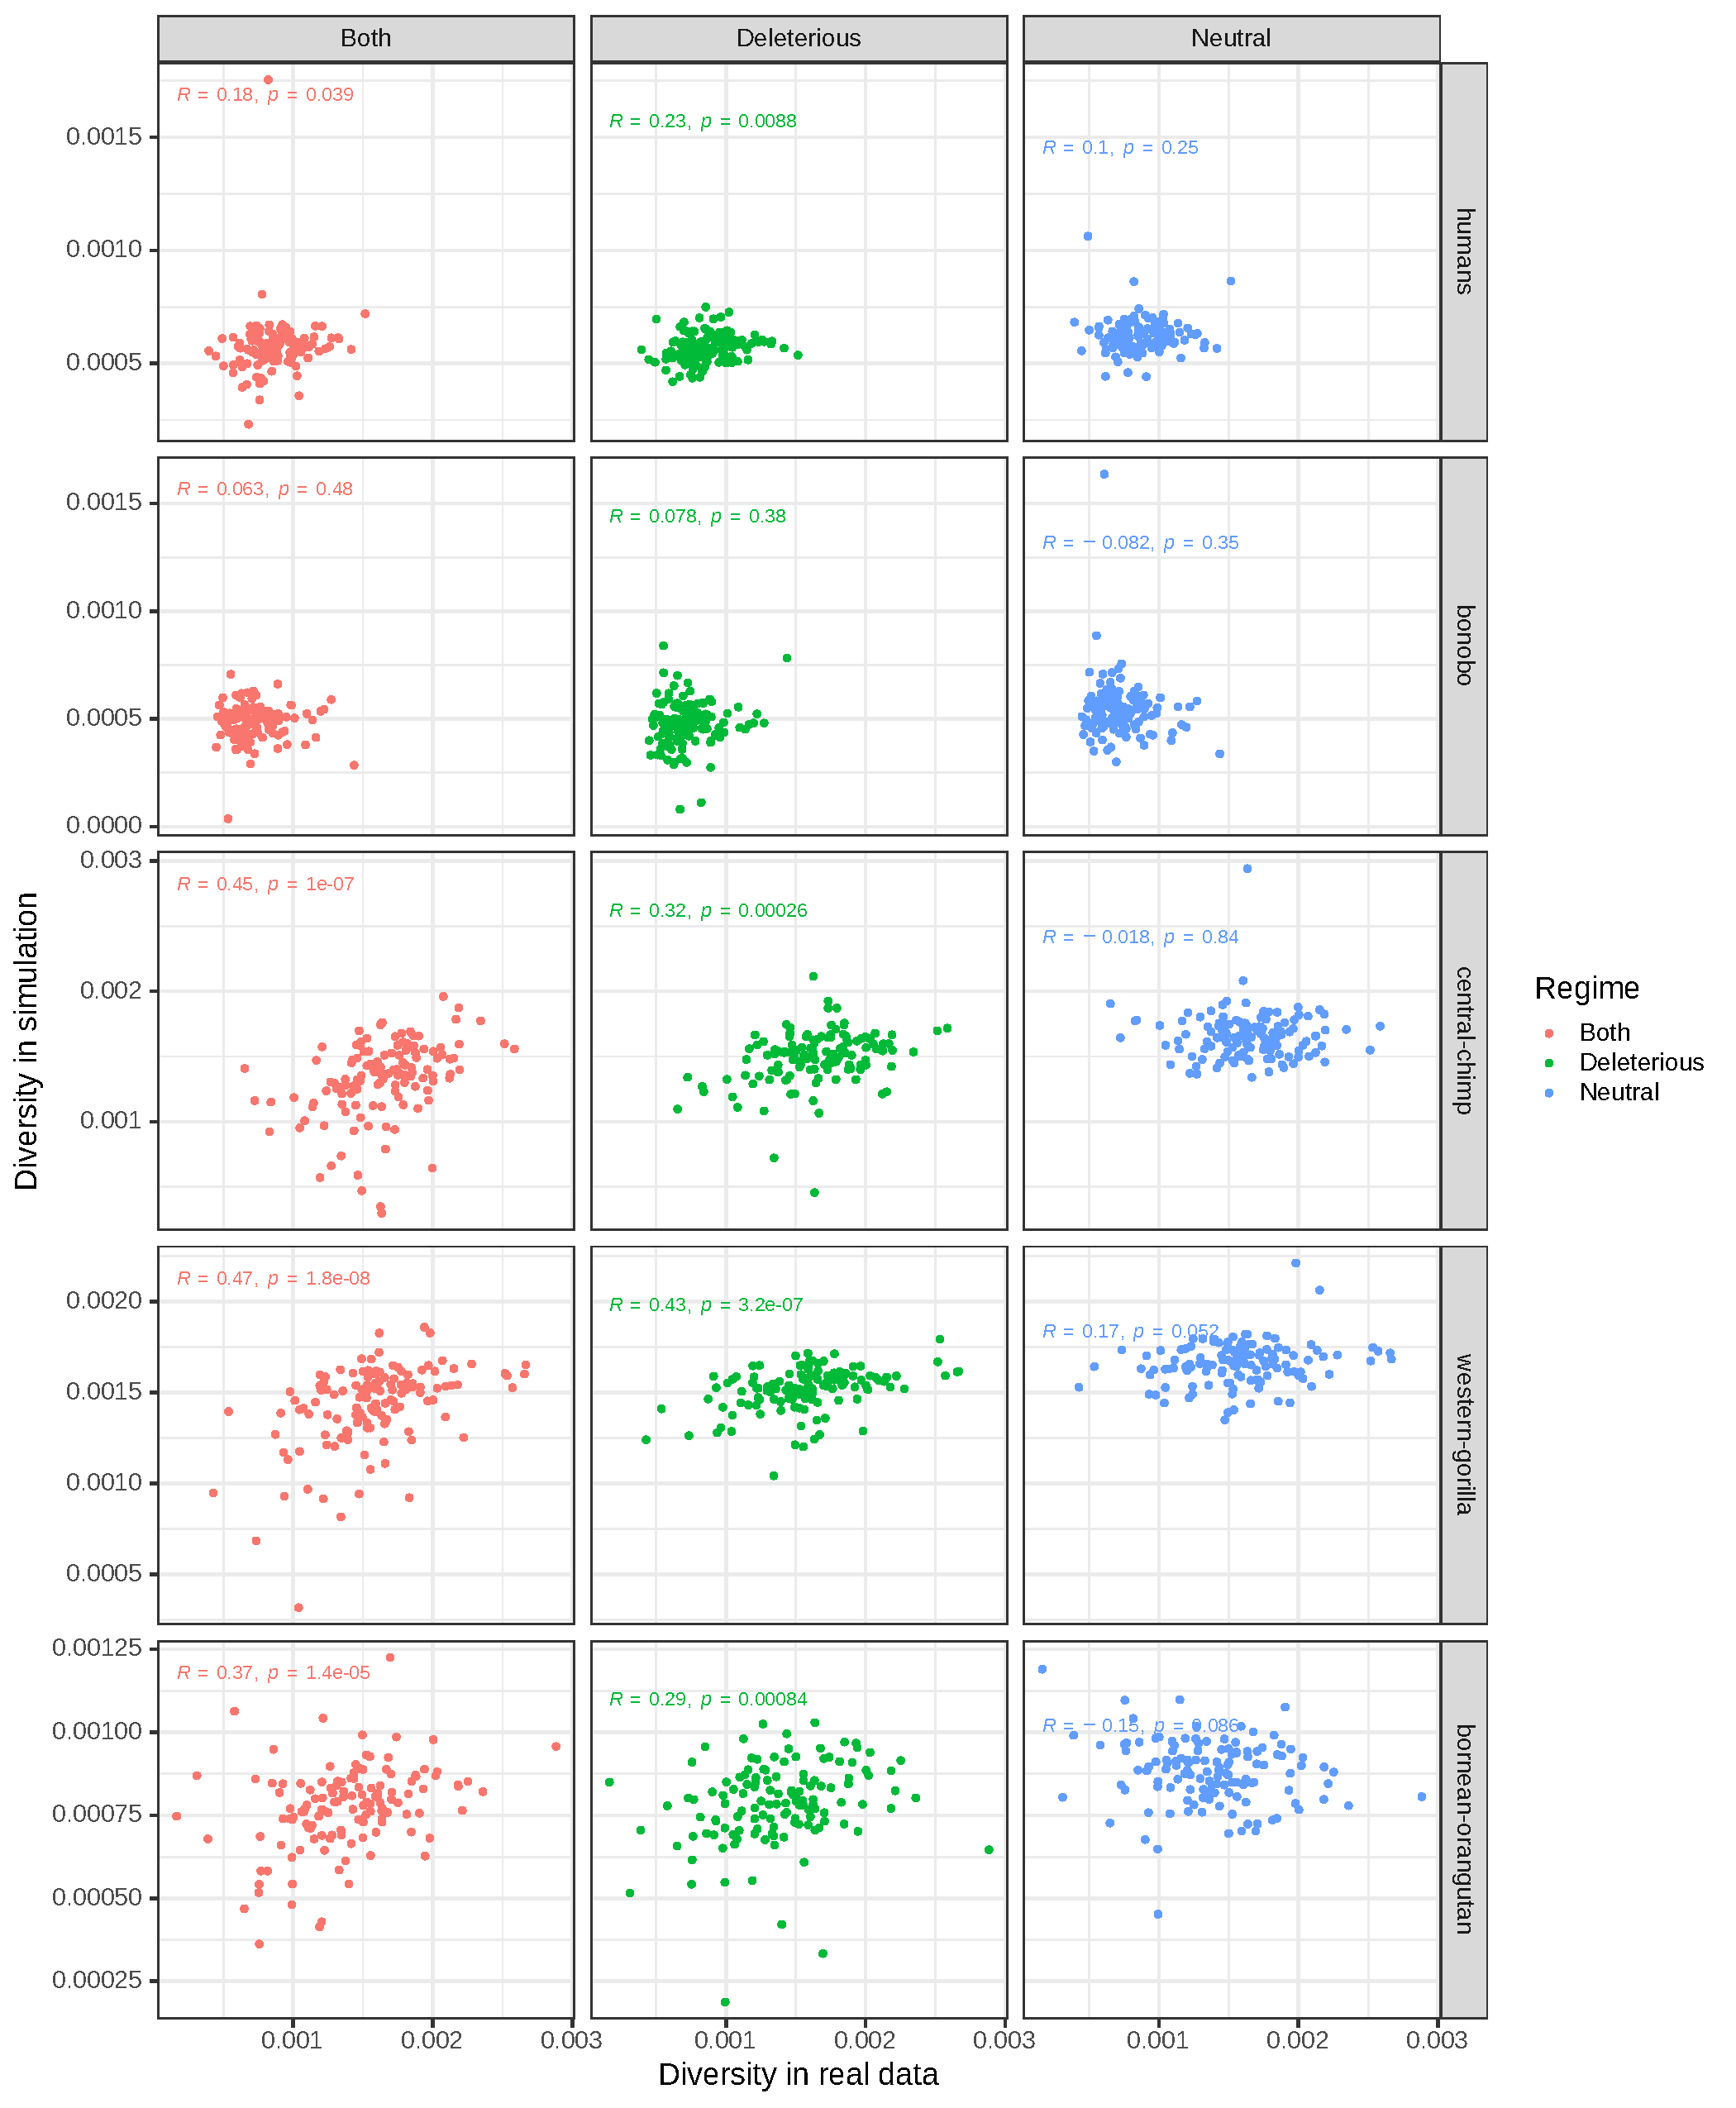
\includegraphics[width=\linewidth]{{figures/data-and-sims_corrs.pdf}}
\centering
\caption{
Scatterplots of genetic diversity in the real great apes data against diversity seen in simulations.
Simulation with deleterious mutations had $\mu_n=\exp{1.4}{-8}$, and the simulation with both deleterious and beneficial mutations had $\mu_n=\exp{1.4}{-8}$ and $\mu_p=\exp{1}{-12}$.
}
\label{fig:data_sims_corrs}
\end{figure}

\begin{figure}[htp]
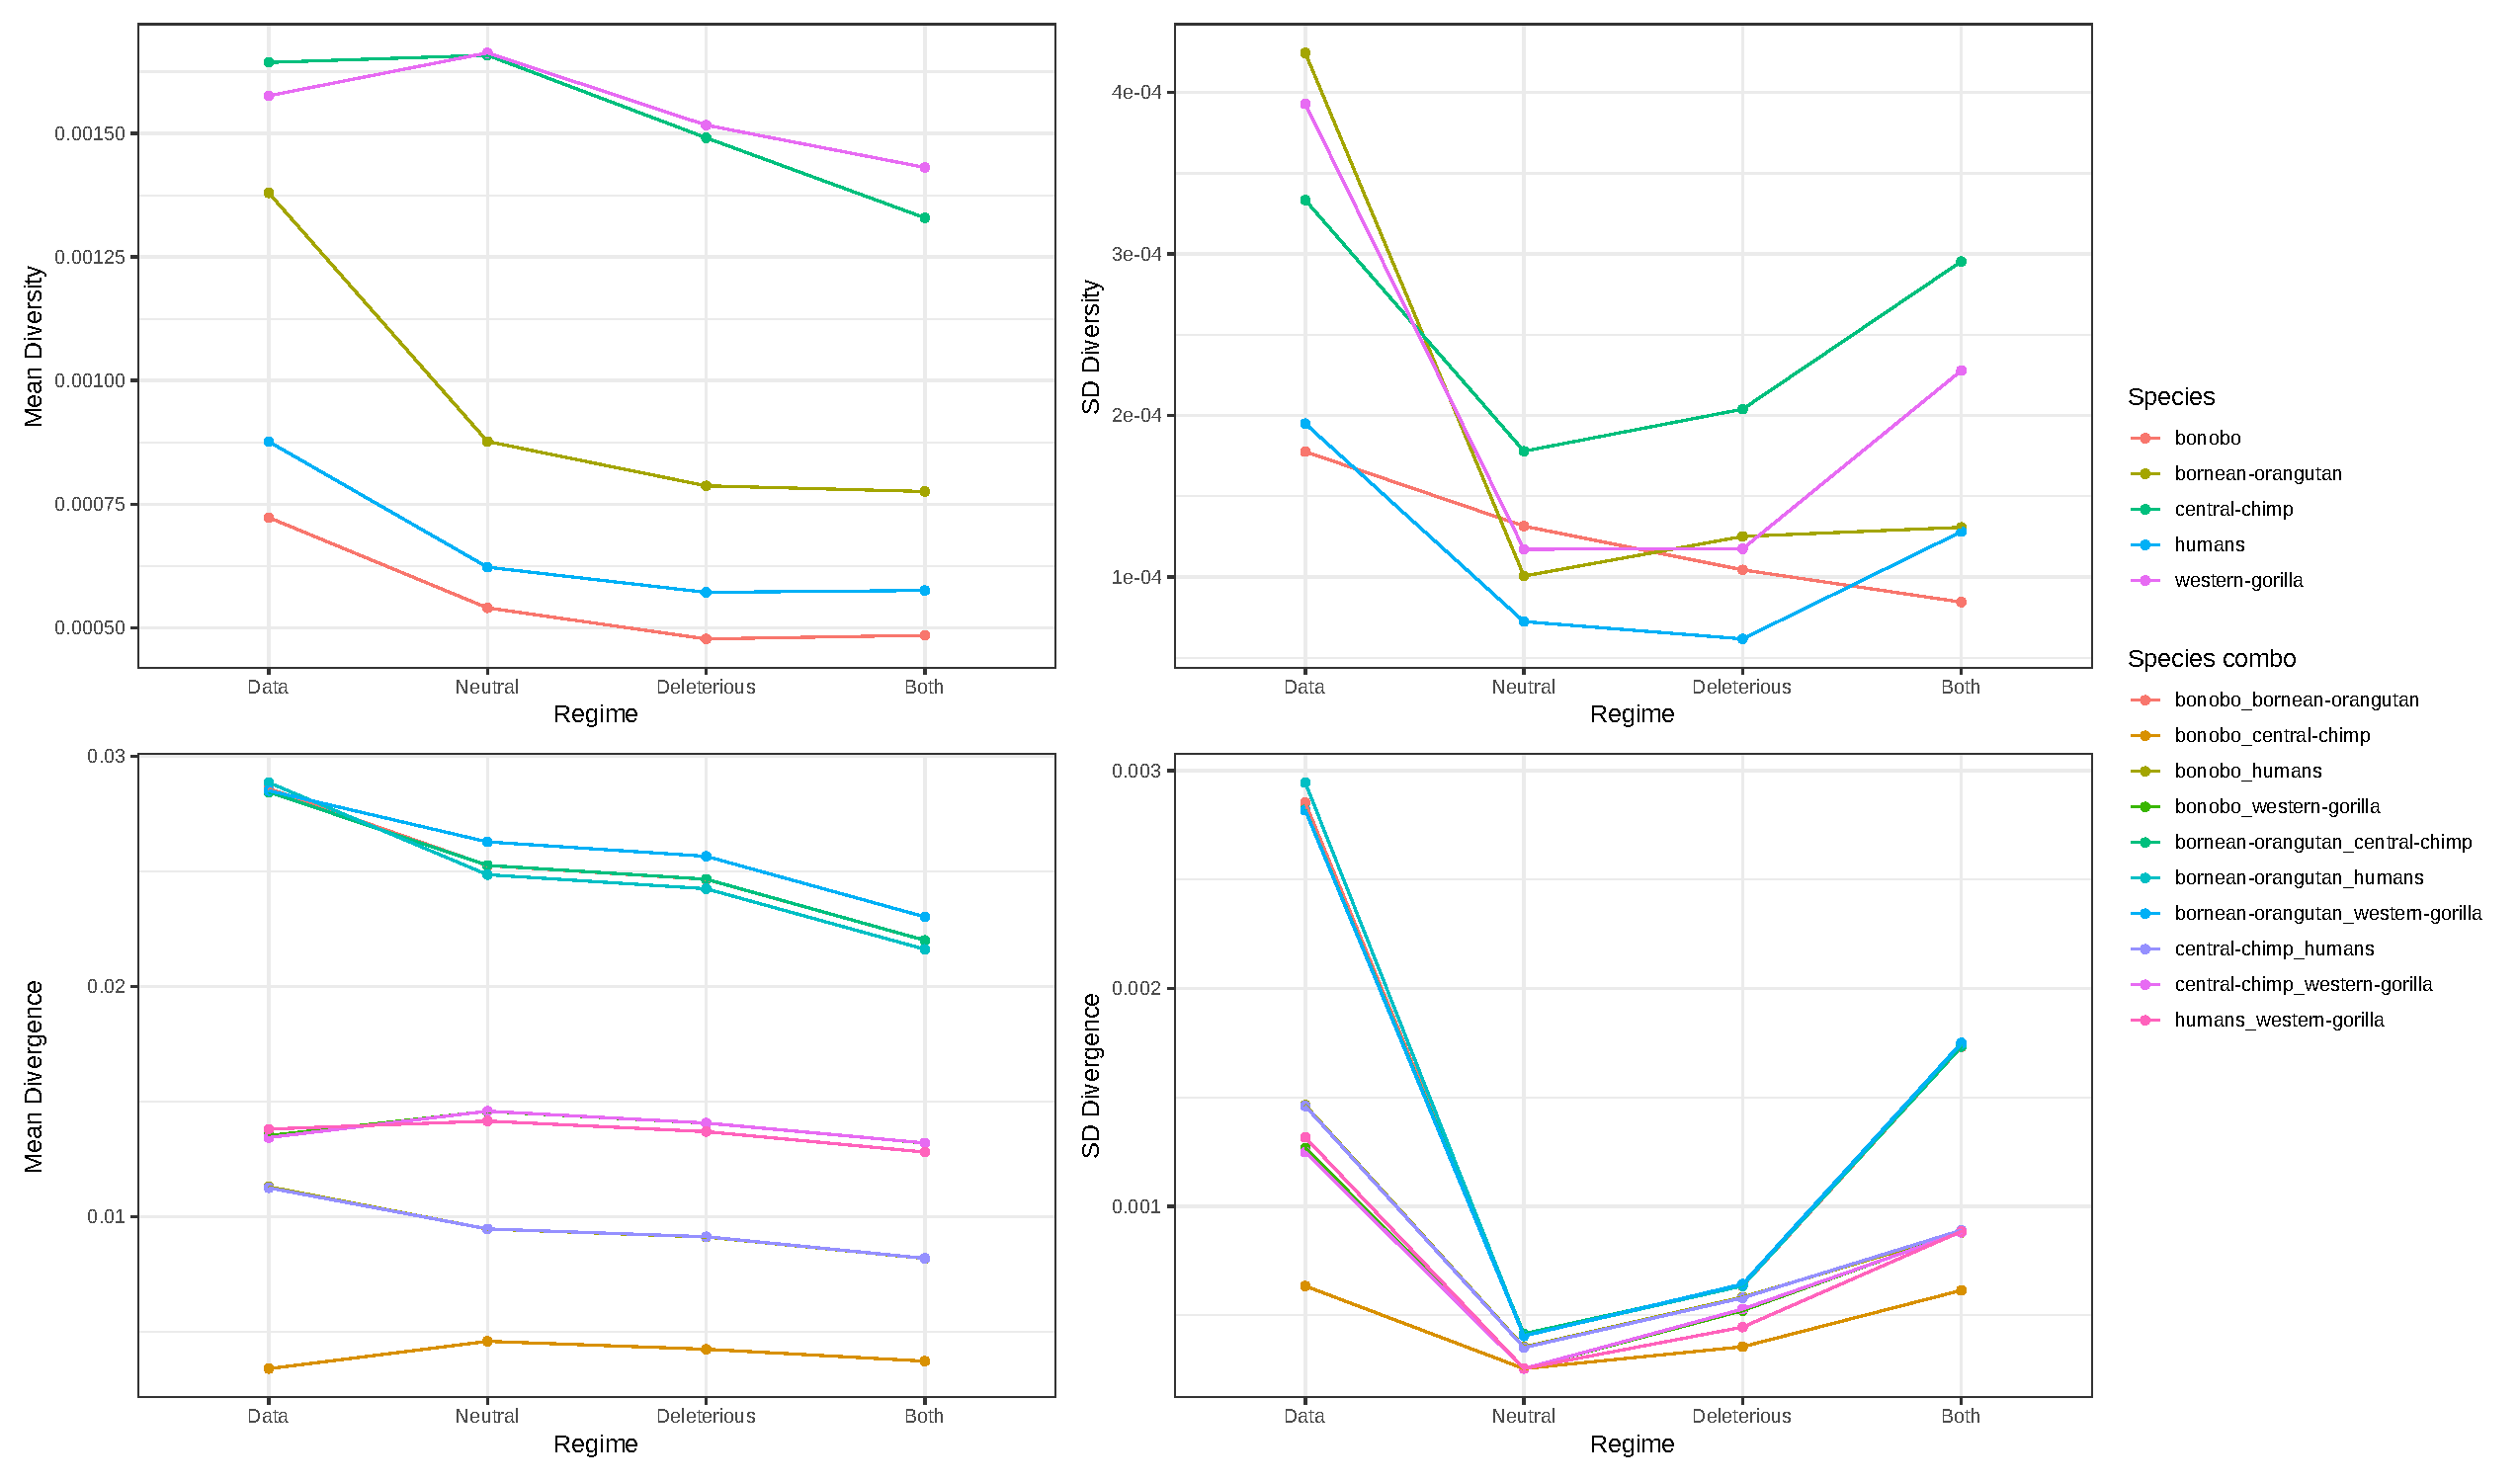
\includegraphics[width=\linewidth]{{figures/data-and-sims_summaries.pdf}}
\centering
\caption{
Summaries of genetic diversity (top) and divergence (bottom) across all species for the data and simulations.
Mean is shown on the left and standard deviation on the right.
``Neutral'' refers to the simulation without any selection,
``Deleterious'' refers to the simulation with deleterious mutations ocurring at a rate of $\expnumber{1.4}{-8}$,
``Both'' refers to the simulation with both beneficial and deleterious mutations, with rates $\expnumber{1}{-12}$ and $\expnumber{1.4}{-8}$ respectively.
}
\label{fig:data_sims_summaries}
\end{figure}


\begin{figure}[htp]
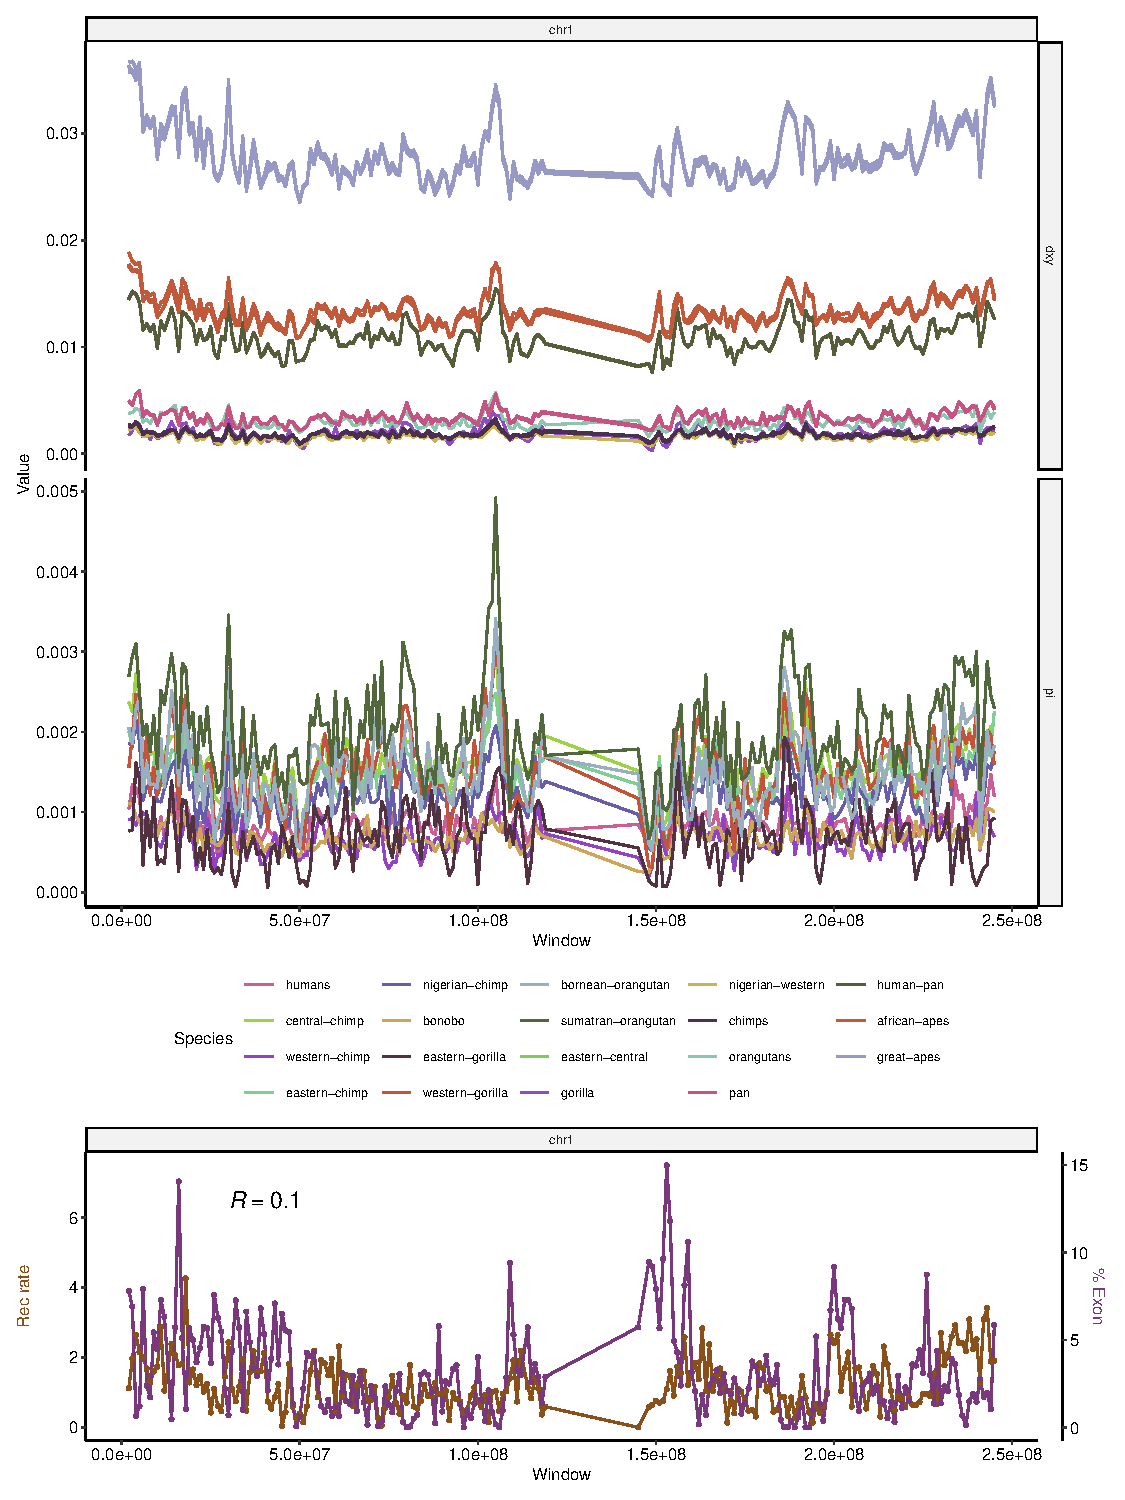
\includegraphics[width=\linewidth]{{figures/all-landscapes_chr1_win-size_1000000_merged-mask_True_state_all_curr_all_prop-acc_0.4.pdf}}
\centering
\caption{
Landscapes of diversity, divergence, exon density and recombination rate across chromosome 1.
See \lcref{fig:chr12_landscapes} for more details.
}
\label{fig:chr1_land}
\end{figure}

\begin{figure}[htp]
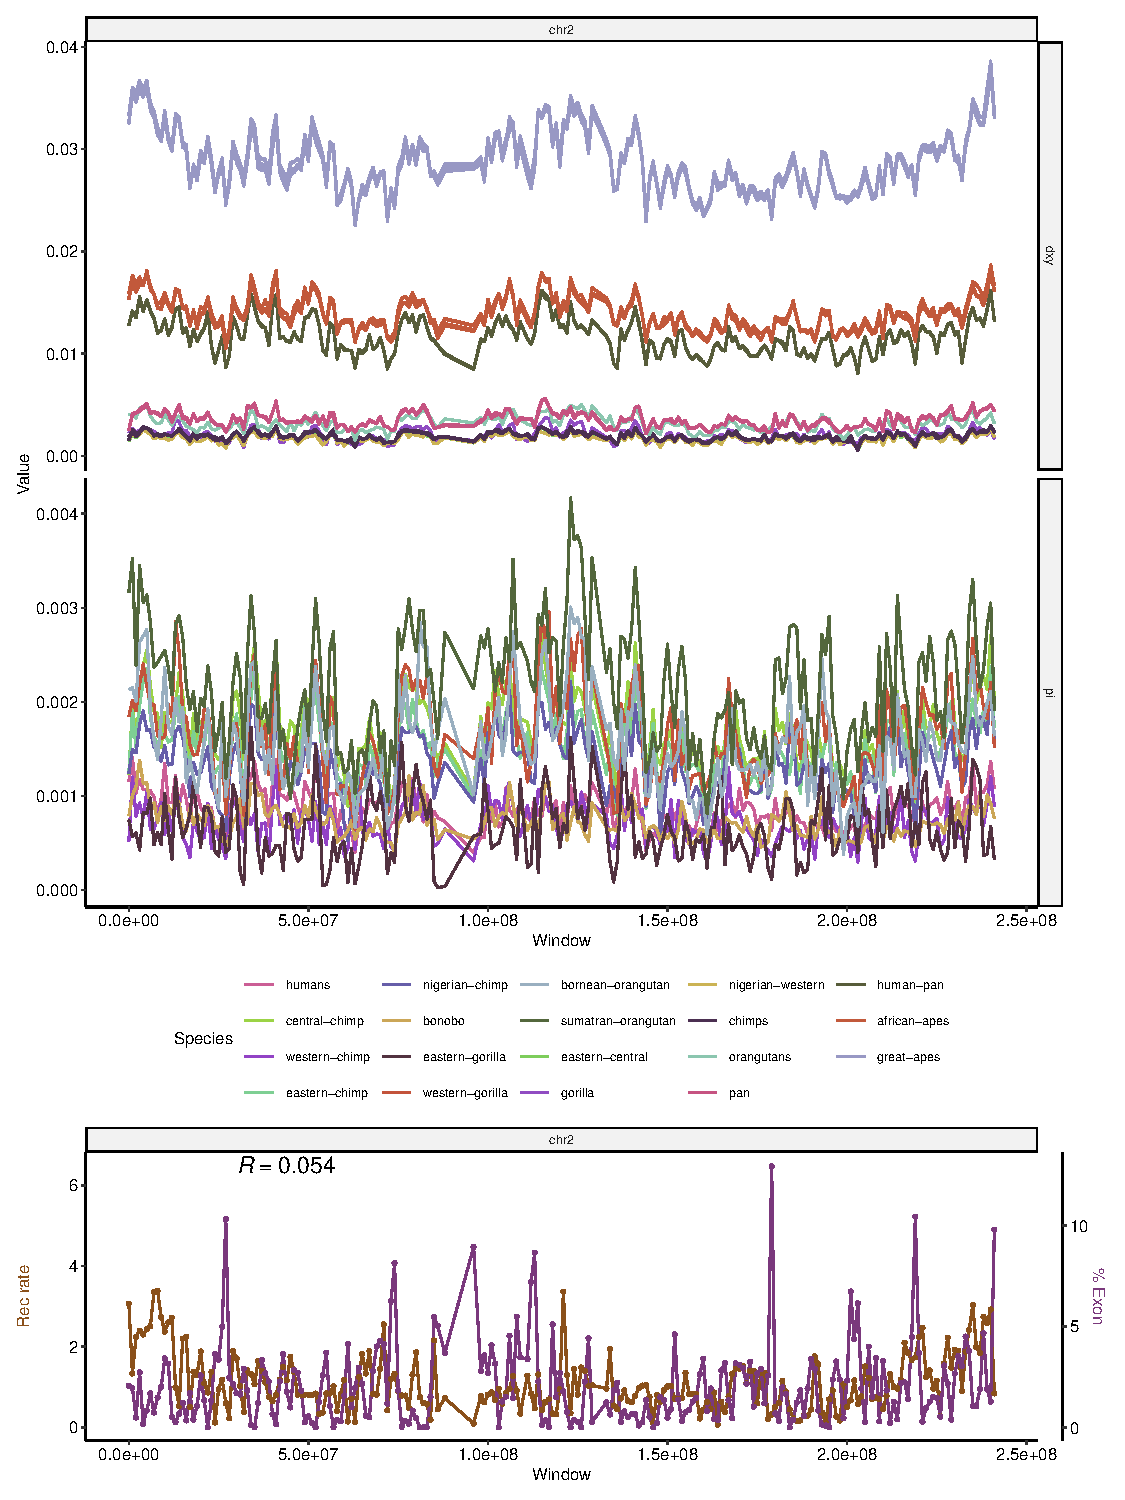
\includegraphics[width=\linewidth]{{figures/all-landscapes_chr2_win-size_1000000_merged-mask_True_state_all_curr_all_prop-acc_0.4.pdf}}
\centering
\caption{
Landscapes of diversity, divergence, exon density and recombination rate across chromosome 2.
See \lcref{fig:chr12_landscapes} for more details.
}
\label{fig:chr2_land}
\end{figure}

\begin{figure}[htp]
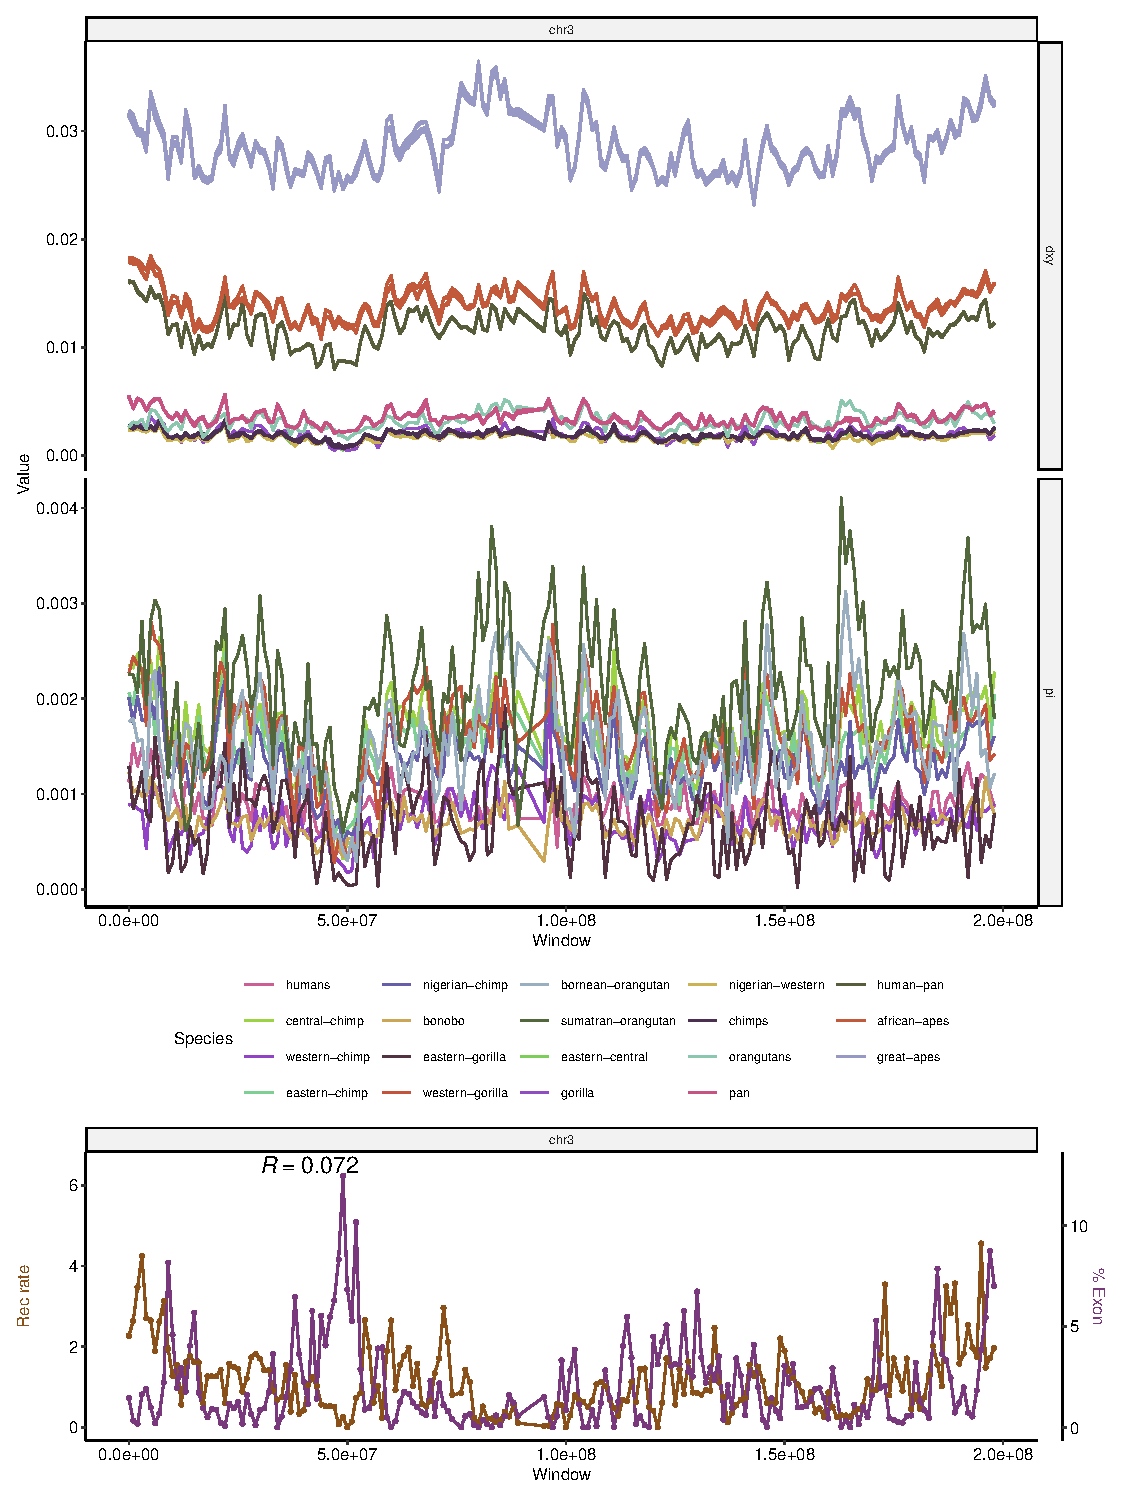
\includegraphics[width=\linewidth]{{figures/all-landscapes_chr3_win-size_1000000_merged-mask_True_state_all_curr_all_prop-acc_0.4.pdf}}
\centering
\caption{
Landscapes of diversity, divergence, exon density and recombination rate across chromosome 3.
See \lcref{fig:chr12_landscapes} for more details.
}
\label{fig:chr3_land}
\end{figure}

\begin{figure}[htp]
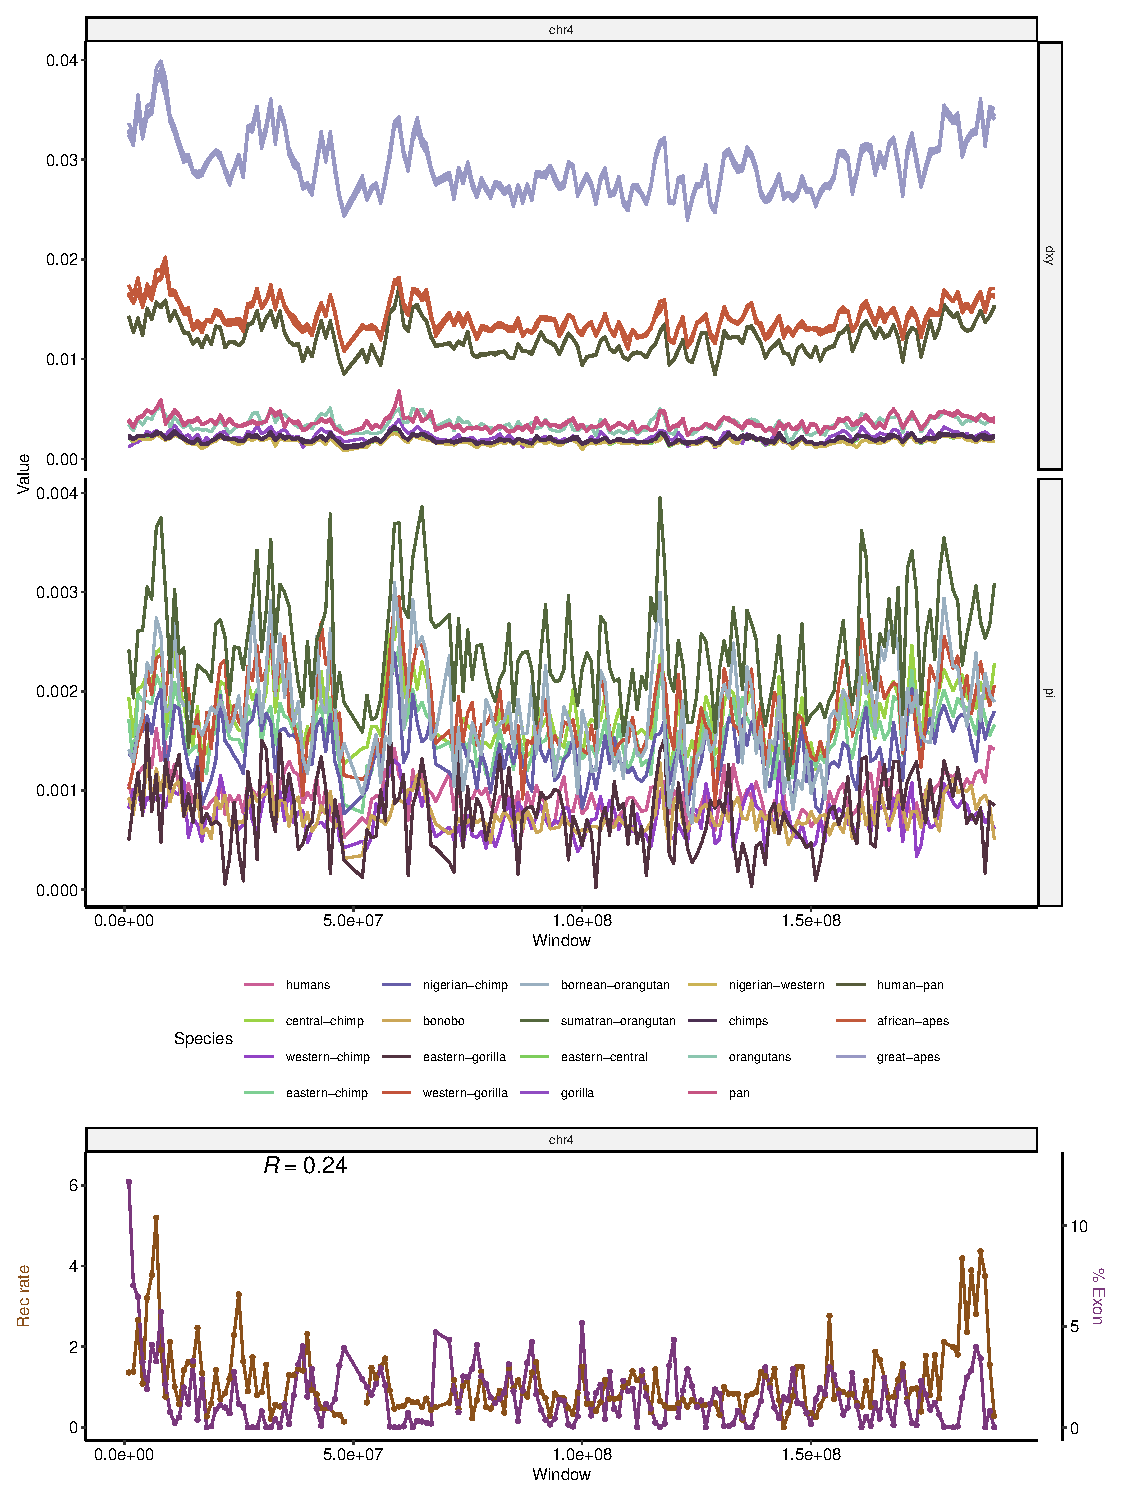
\includegraphics[width=\linewidth]{{figures/all-landscapes_chr4_win-size_1000000_merged-mask_True_state_all_curr_all_prop-acc_0.4.pdf}}
\centering
\caption{
Landscapes of diversity, divergence, exon density and recombination rate across chromosome 4.
See \lcref{fig:chr12_landscapes} for more details.
}
\label{fig:chr4_land}
\end{figure}

\begin{figure}[htp]
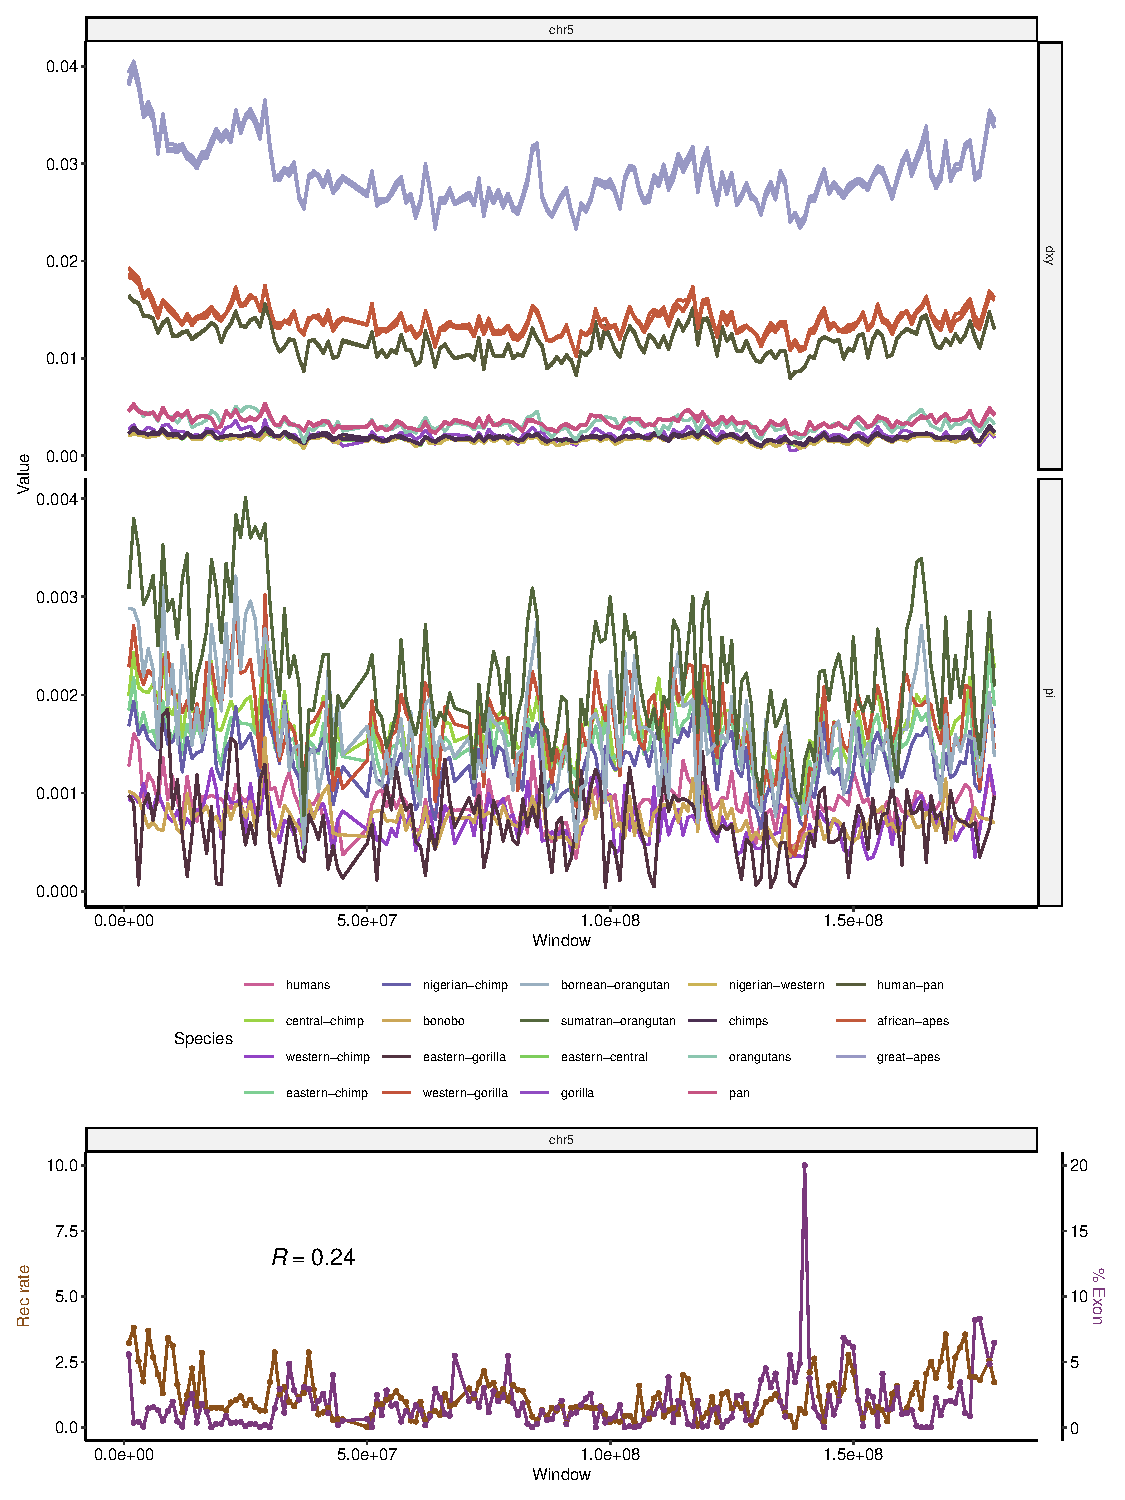
\includegraphics[width=\linewidth]{{figures/all-landscapes_chr5_win-size_1000000_merged-mask_True_state_all_curr_all_prop-acc_0.4.pdf}}
\centering
\caption{
Landscapes of diversity, divergence, exon density and recombination rate across chromosome 5.
See \lcref{fig:chr12_landscapes} for more details.
}
\label{fig:chr5_land}
\end{figure}

\begin{figure}[htp]
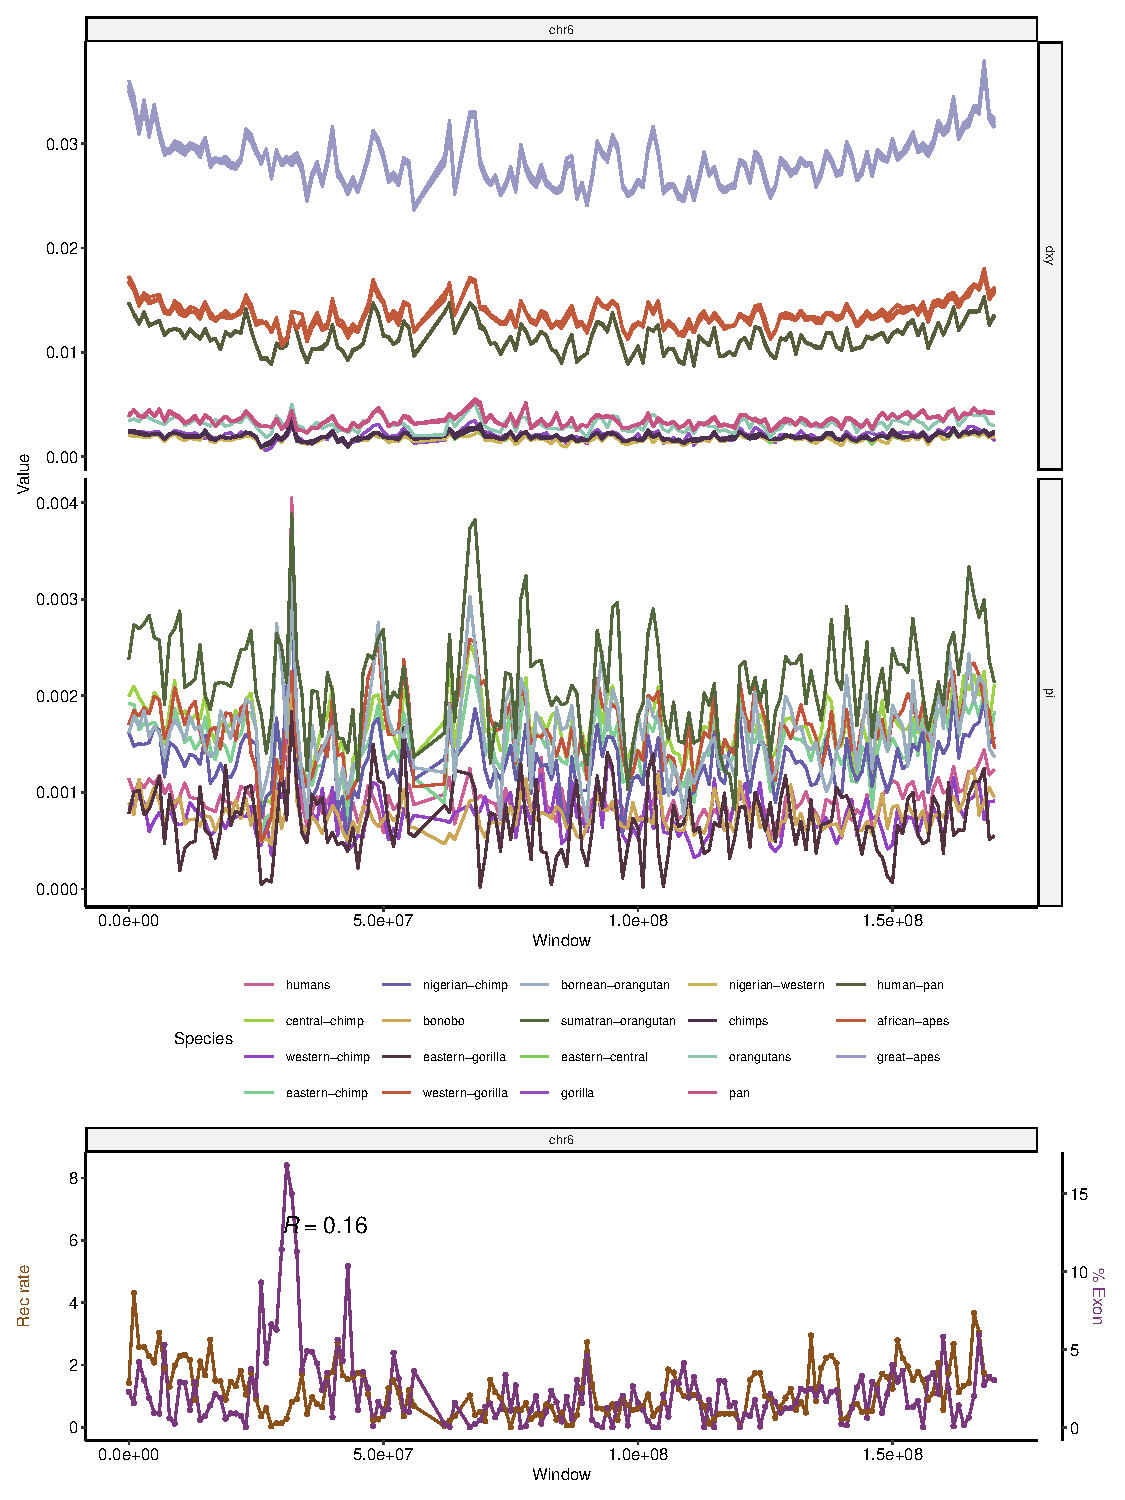
\includegraphics[width=\linewidth]{{figures/all-landscapes_chr6_win-size_1000000_merged-mask_True_state_all_curr_all_prop-acc_0.4.pdf}}
\centering
\caption{
Landscapes of diversity, divergence, exon density and recombination rate across chromosome 6.
See \lcref{fig:chr12_landscapes} for more details.
}
\label{fig:chr6_land}
\end{figure}

\begin{figure}[htp]
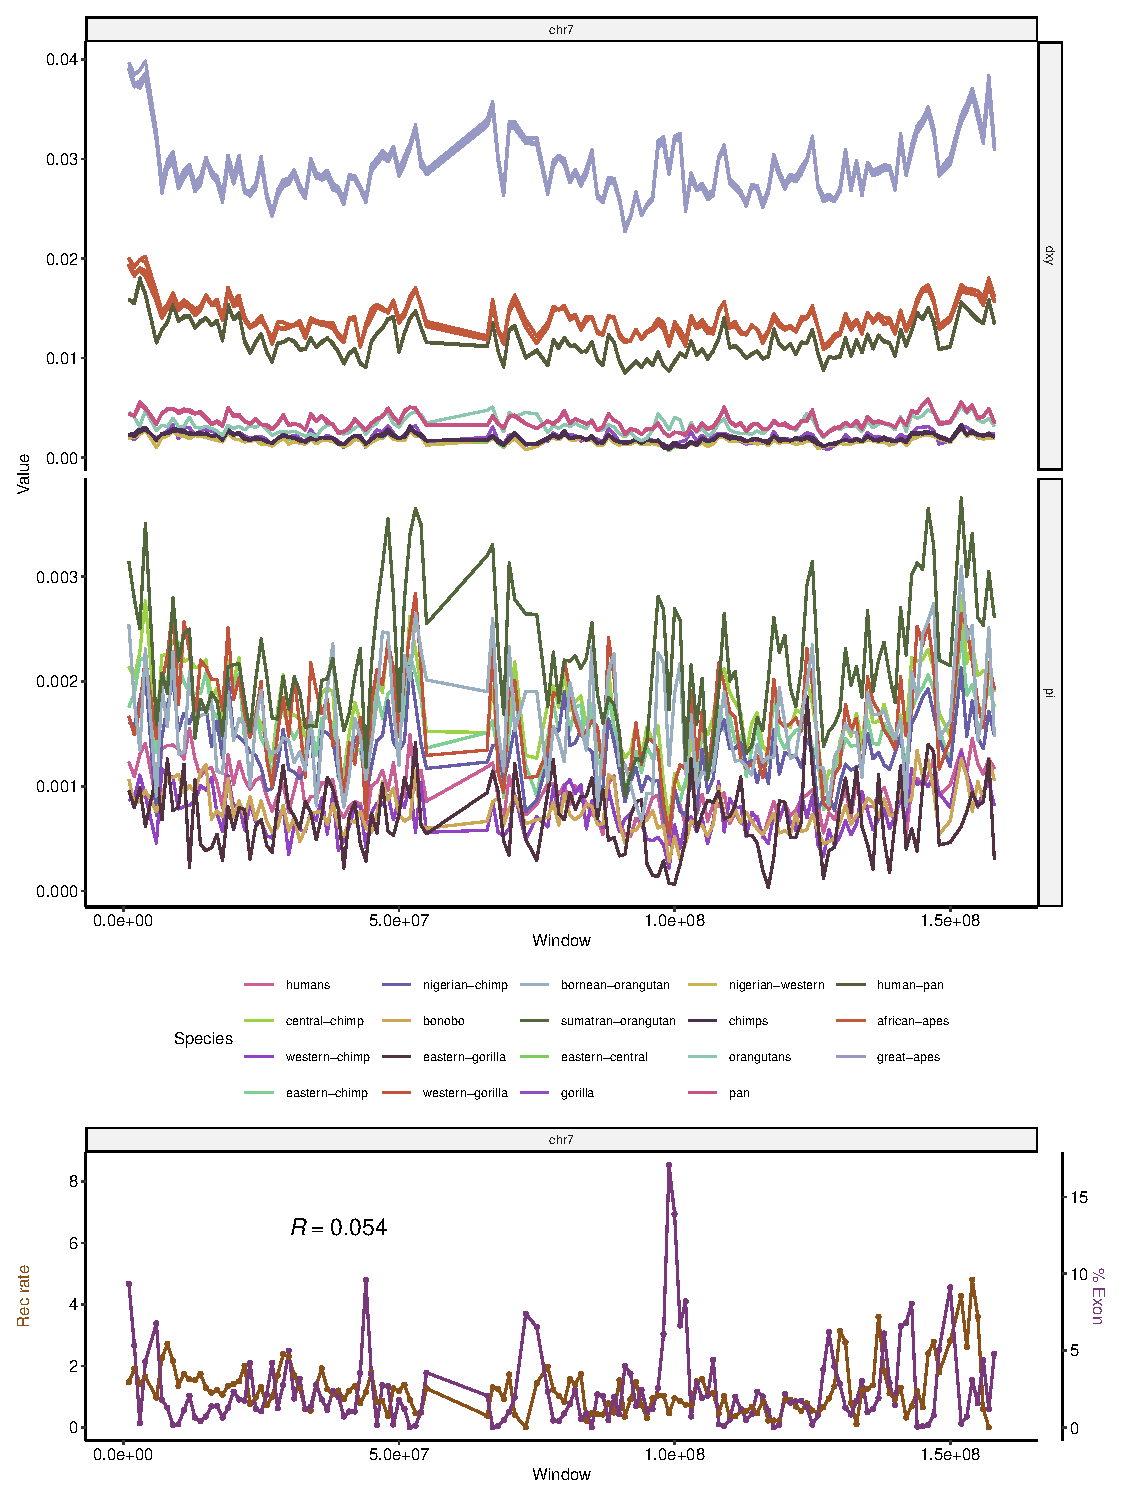
\includegraphics[width=\linewidth]{{figures/all-landscapes_chr7_win-size_1000000_merged-mask_True_state_all_curr_all_prop-acc_0.4.pdf}}
\centering
\caption{
Landscapes of diversity, divergence, exon density and recombination rate across chromosome 7.
See \lcref{fig:chr12_landscapes} for more details.
}
\label{fig:chr7_land}
\end{figure}

\begin{figure}[htp]
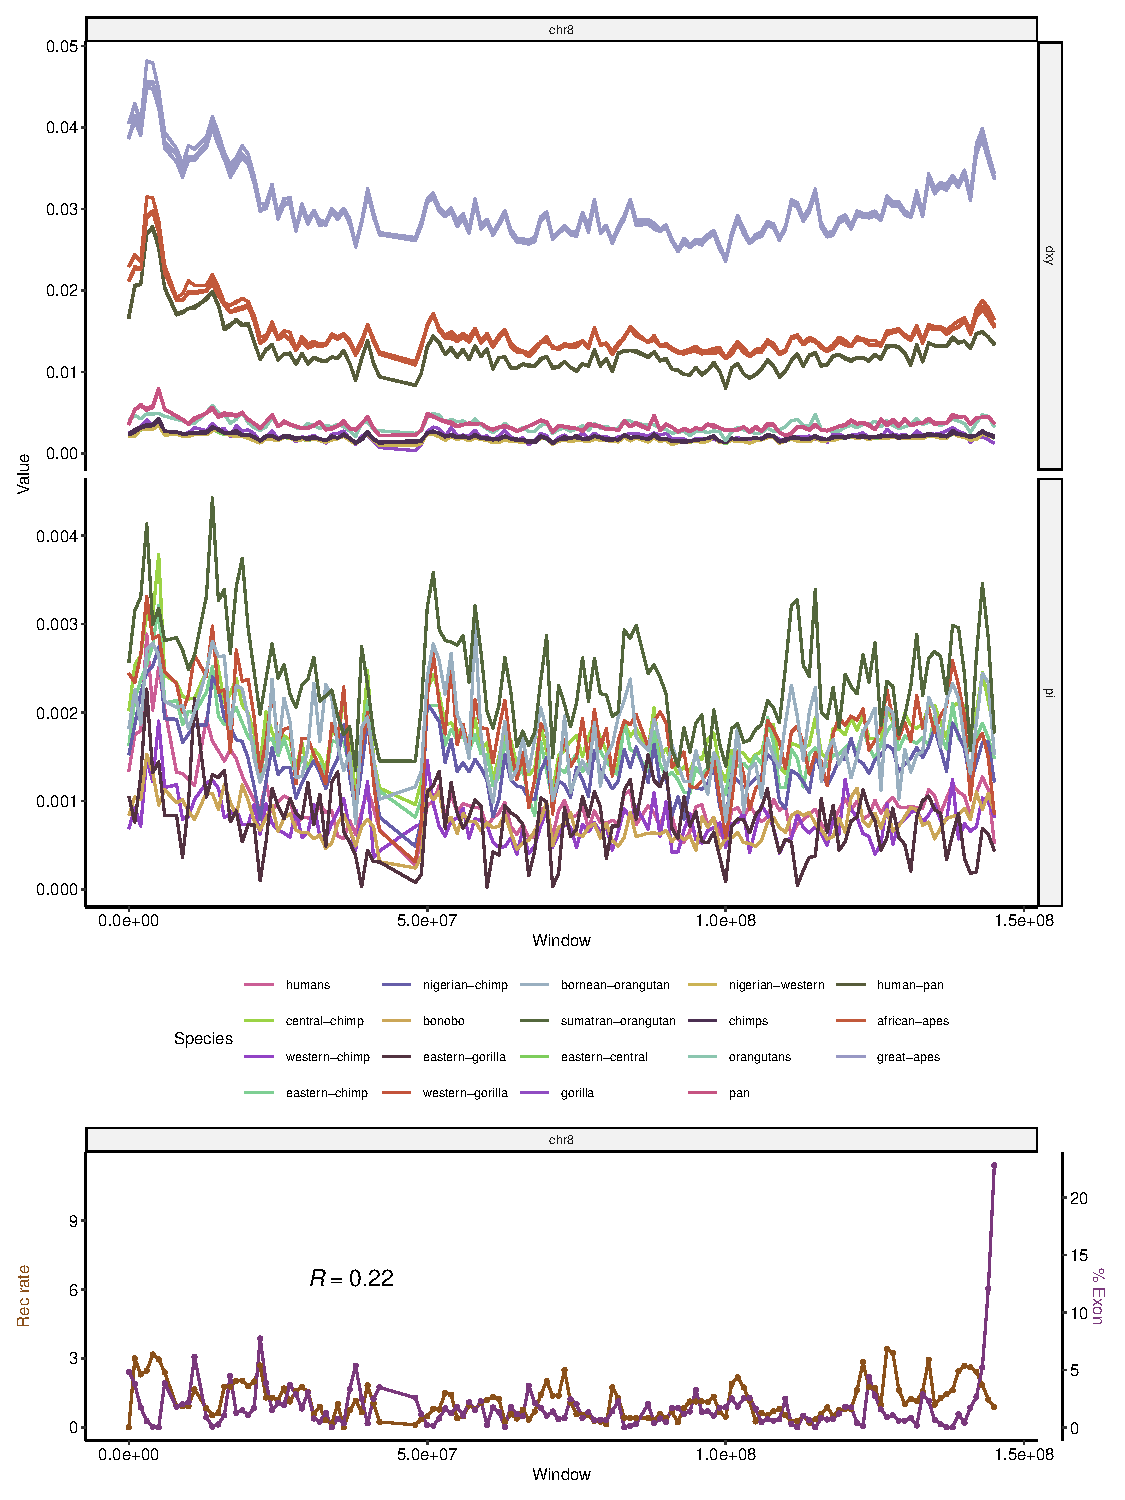
\includegraphics[width=\linewidth]{{figures/all-landscapes_chr8_win-size_1000000_merged-mask_True_state_all_curr_all_prop-acc_0.4.pdf}}
\centering
\caption{
Landscapes of diversity, divergence, exon density and recombination rate across chromosome 8.
See \lcref{fig:chr12_landscapes} for more details.
}
\label{fig:chr8_land}
\end{figure}

\begin{figure}[htp]
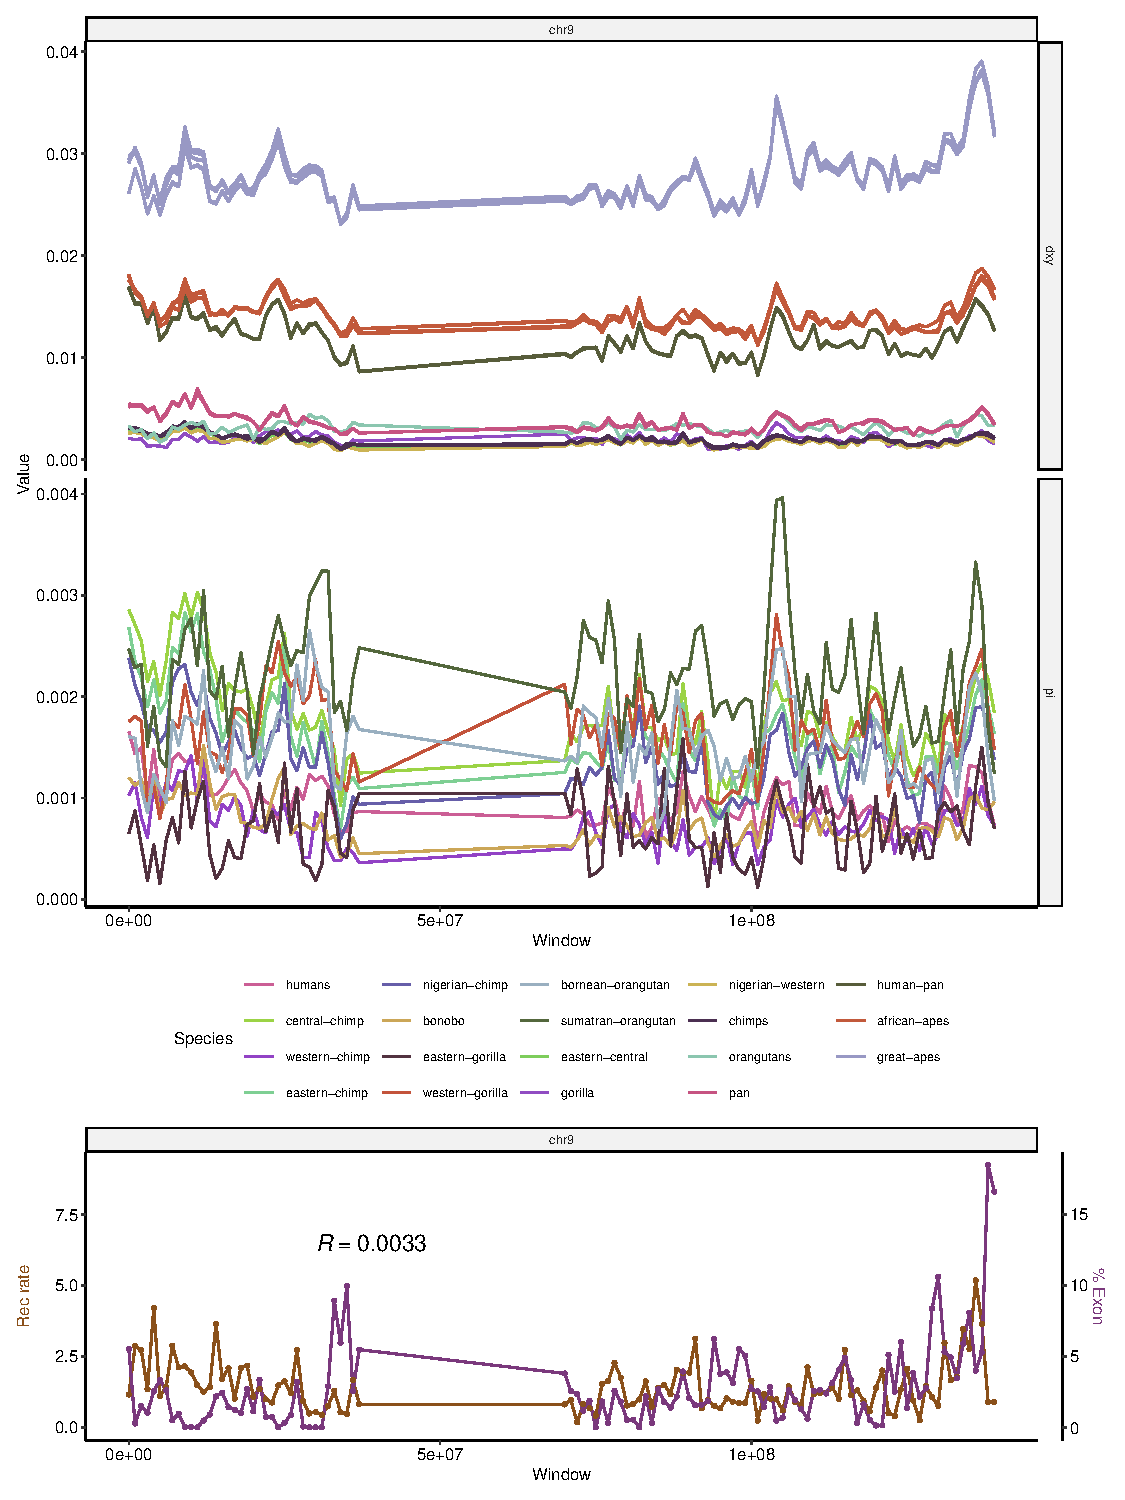
\includegraphics[width=\linewidth]{{figures/all-landscapes_chr9_win-size_1000000_merged-mask_True_state_all_curr_all_prop-acc_0.4.pdf}}
\centering
\caption{
Landscapes of diversity, divergence, exon density and recombination rate across chromosome 9.
See \lcref{fig:chr12_landscapes} for more details.
}
\label{fig:chr9_land}
\end{figure}

\begin{figure}[htp]
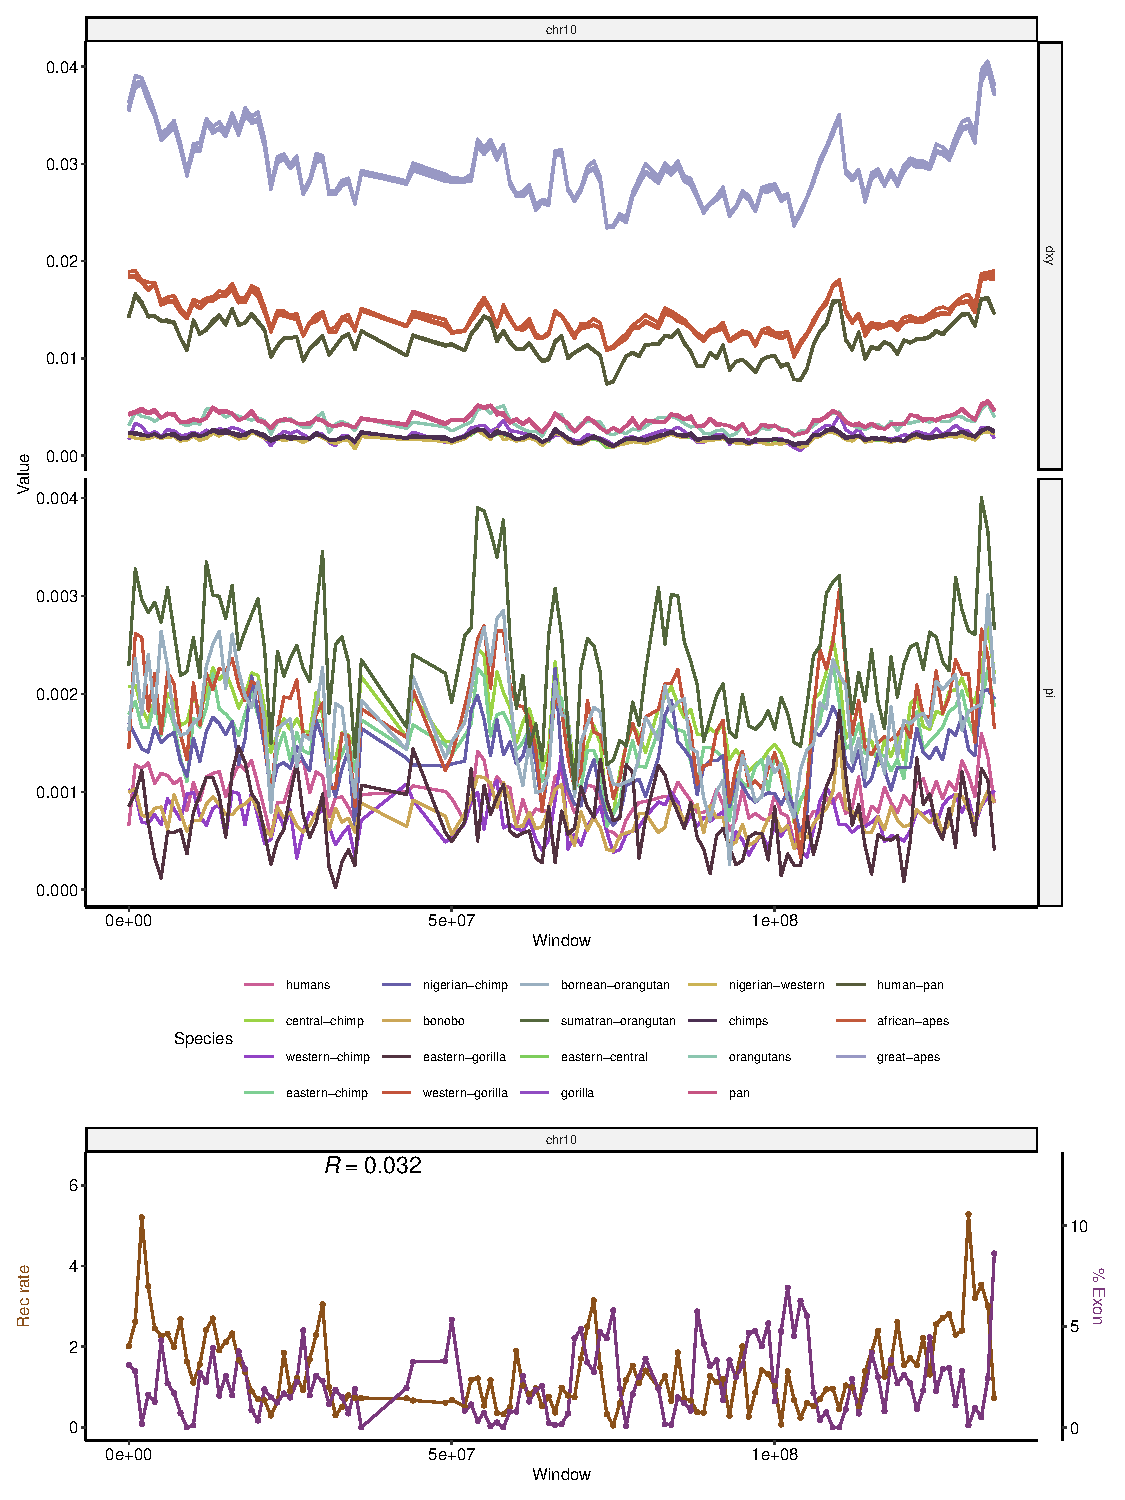
\includegraphics[width=\linewidth]{{figures/all-landscapes_chr10_win-size_1000000_merged-mask_True_state_all_curr_all_prop-acc_0.4.pdf}}
\centering
\caption{
Landscapes of diversity, divergence, exon density and recombination rate across chromosome 10.
See \lcref{fig:chr12_landscapes} for more details.
}
\label{fig:chr10_land}
\end{figure}

\begin{figure}[htp]
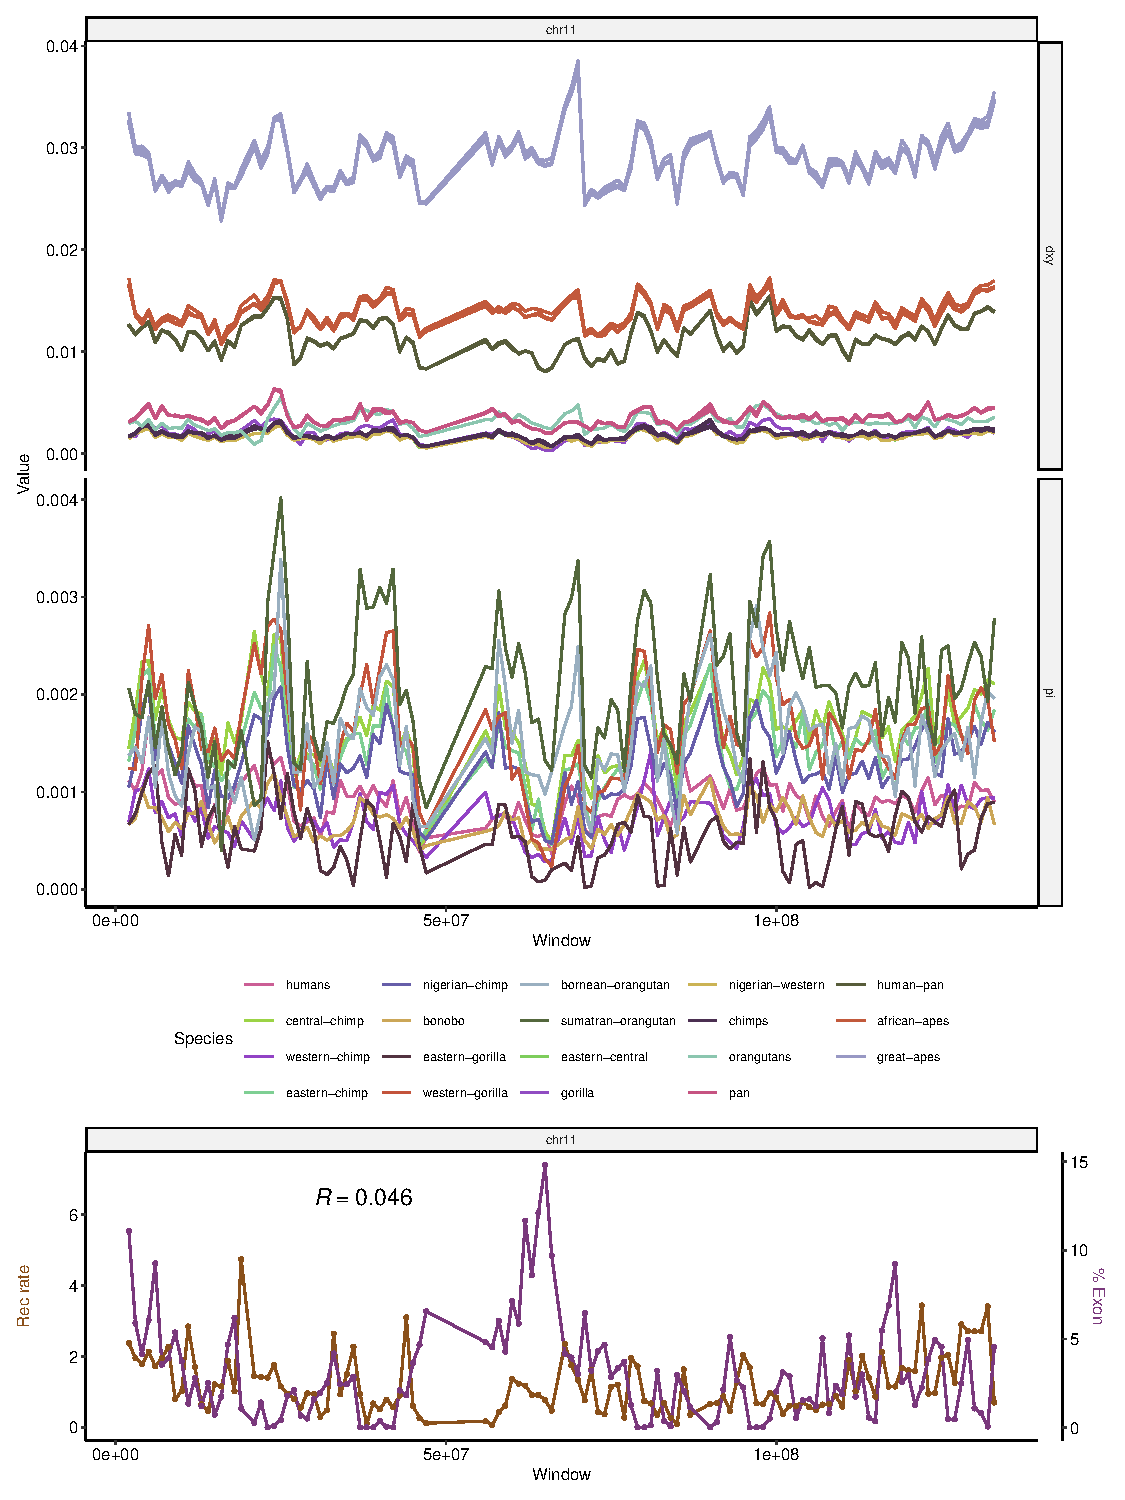
\includegraphics[width=\linewidth]{{figures/all-landscapes_chr11_win-size_1000000_merged-mask_True_state_all_curr_all_prop-acc_0.4.pdf}}
\centering
\caption{
Landscapes of diversity, divergence, exon density and recombination rate across chromosome 11.
See \lcref{fig:chr12_landscapes} for more details.
}
\label{fig:chr11_land}
\end{figure}

\begin{figure}[htp]
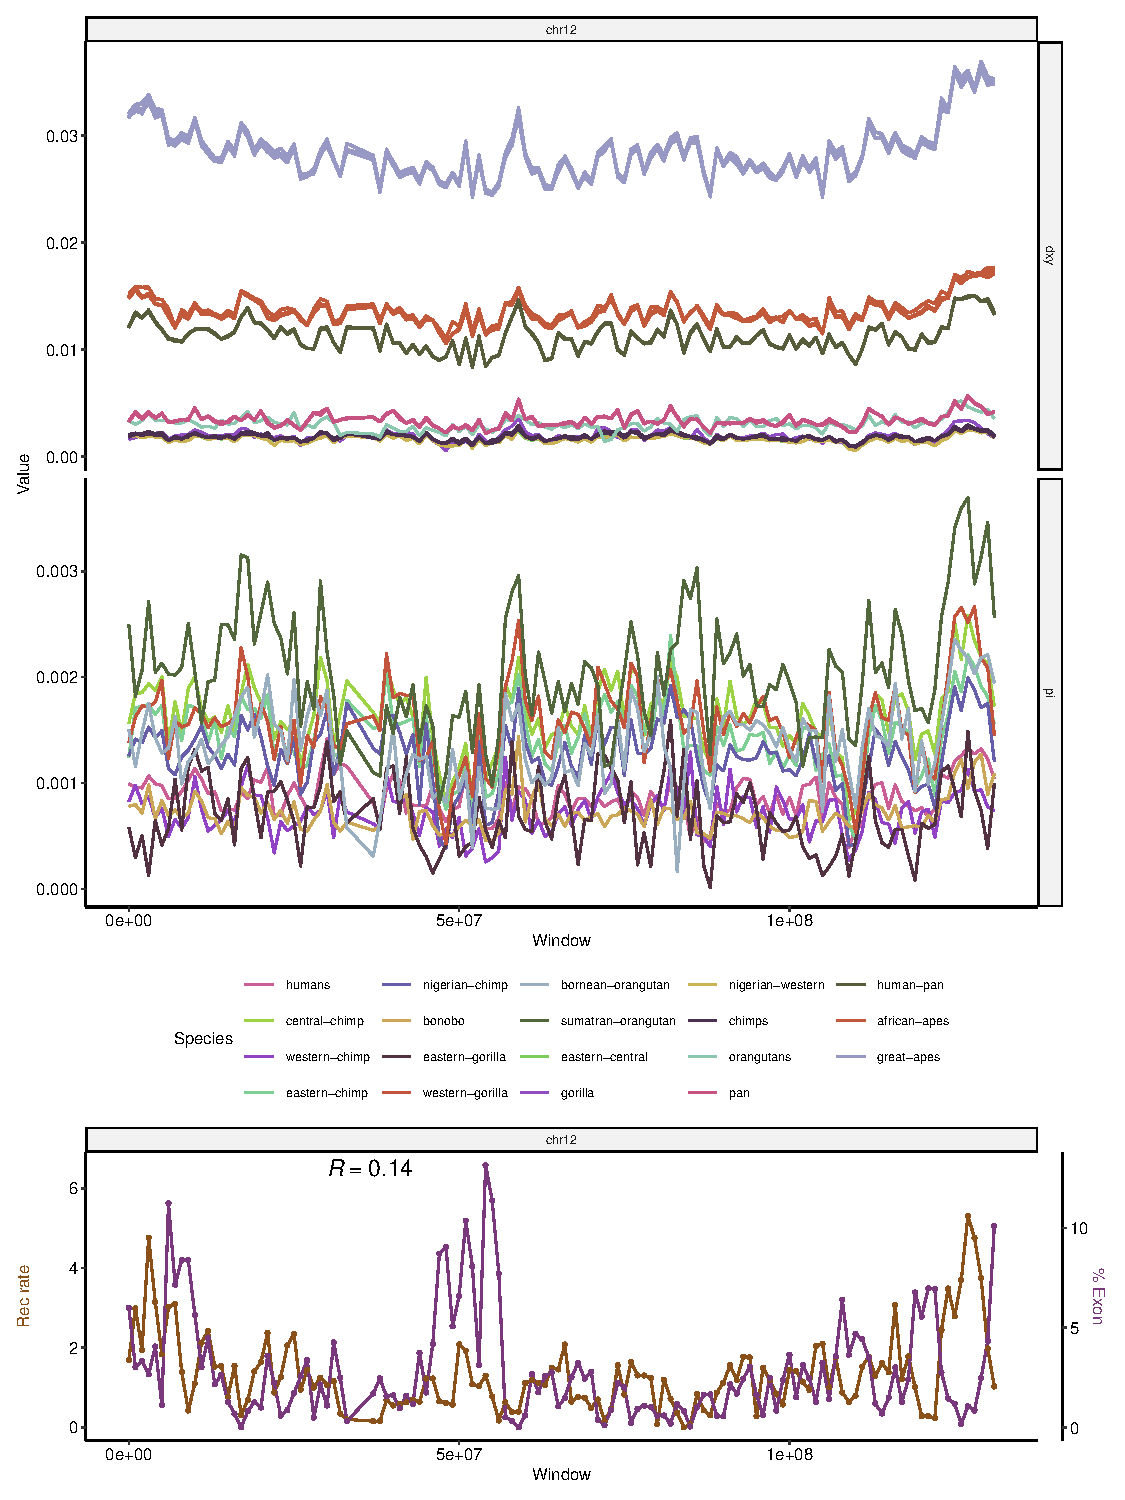
\includegraphics[width=\linewidth]{{figures/all-landscapes_chr12_win-size_1000000_merged-mask_True_state_all_curr_all_prop-acc_0.4.pdf}}
\centering
\caption{
Landscapes of diversity, divergence, exon density and recombination rate across chromosome 12.
See \lcref{fig:chr12_landscapes} for more details.
}
\label{fig:chr12_land}
\end{figure}

\begin{figure}[htp]
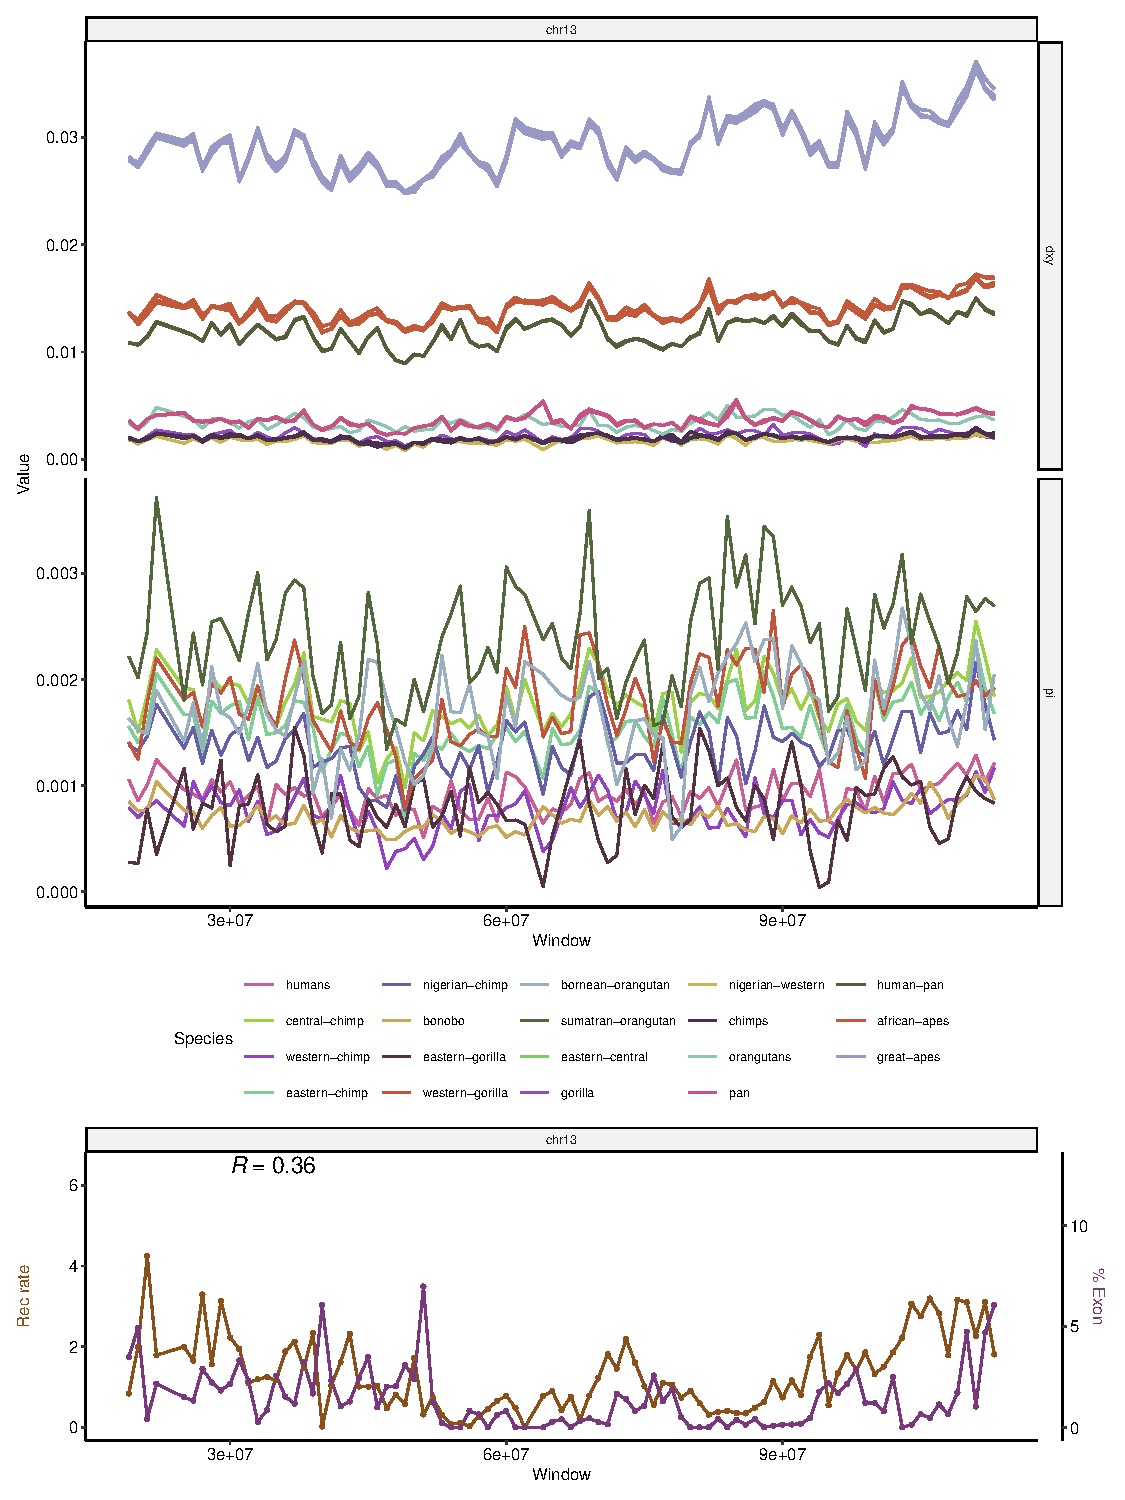
\includegraphics[width=\linewidth]{{figures/all-landscapes_chr13_win-size_1000000_merged-mask_True_state_all_curr_all_prop-acc_0.4.pdf}}
\centering
\caption{
Landscapes of diversity, divergence, exon density and recombination rate across chromosome 13.
See \lcref{fig:chr12_landscapes} for more details.
}
\label{fig:chr13_land}
\end{figure}

\begin{figure}[htp]
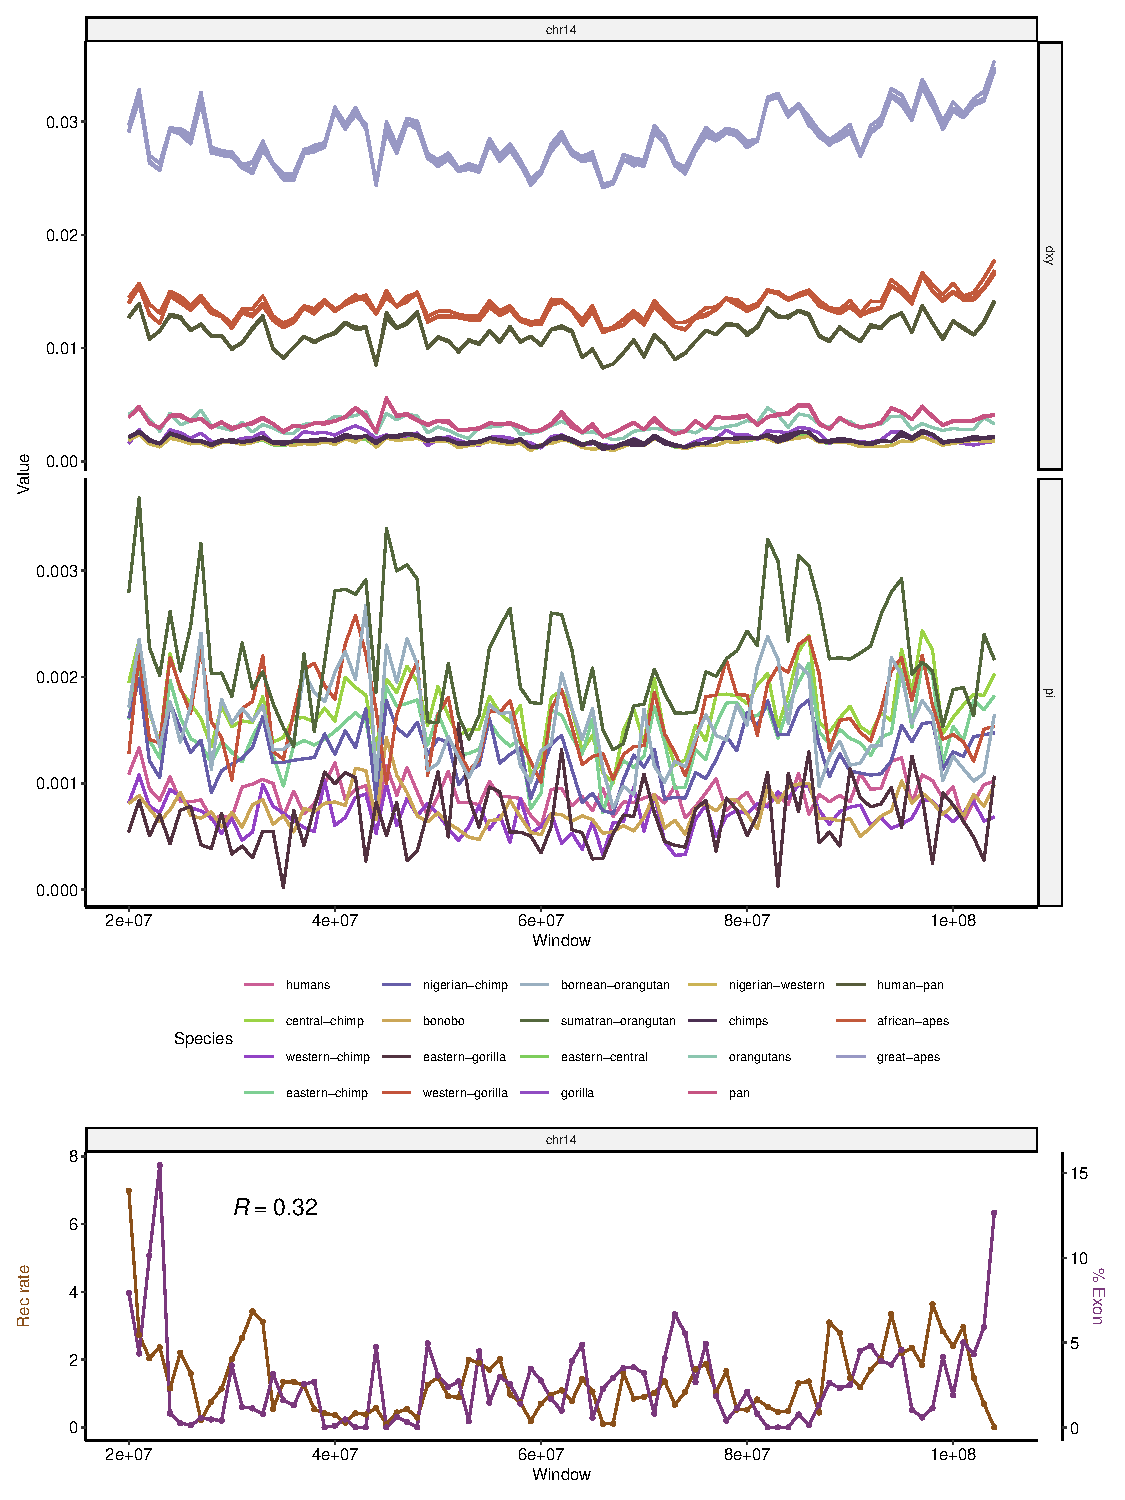
\includegraphics[width=\linewidth]{{figures/all-landscapes_chr14_win-size_1000000_merged-mask_True_state_all_curr_all_prop-acc_0.4.pdf}}
\centering
\caption{
Landscapes of diversity, divergence, exon density and recombination rate across chromosome 14.
See \lcref{fig:chr12_landscapes} for more details.
}
\label{fig:chr14_land}
\end{figure}

\begin{figure}[htp]
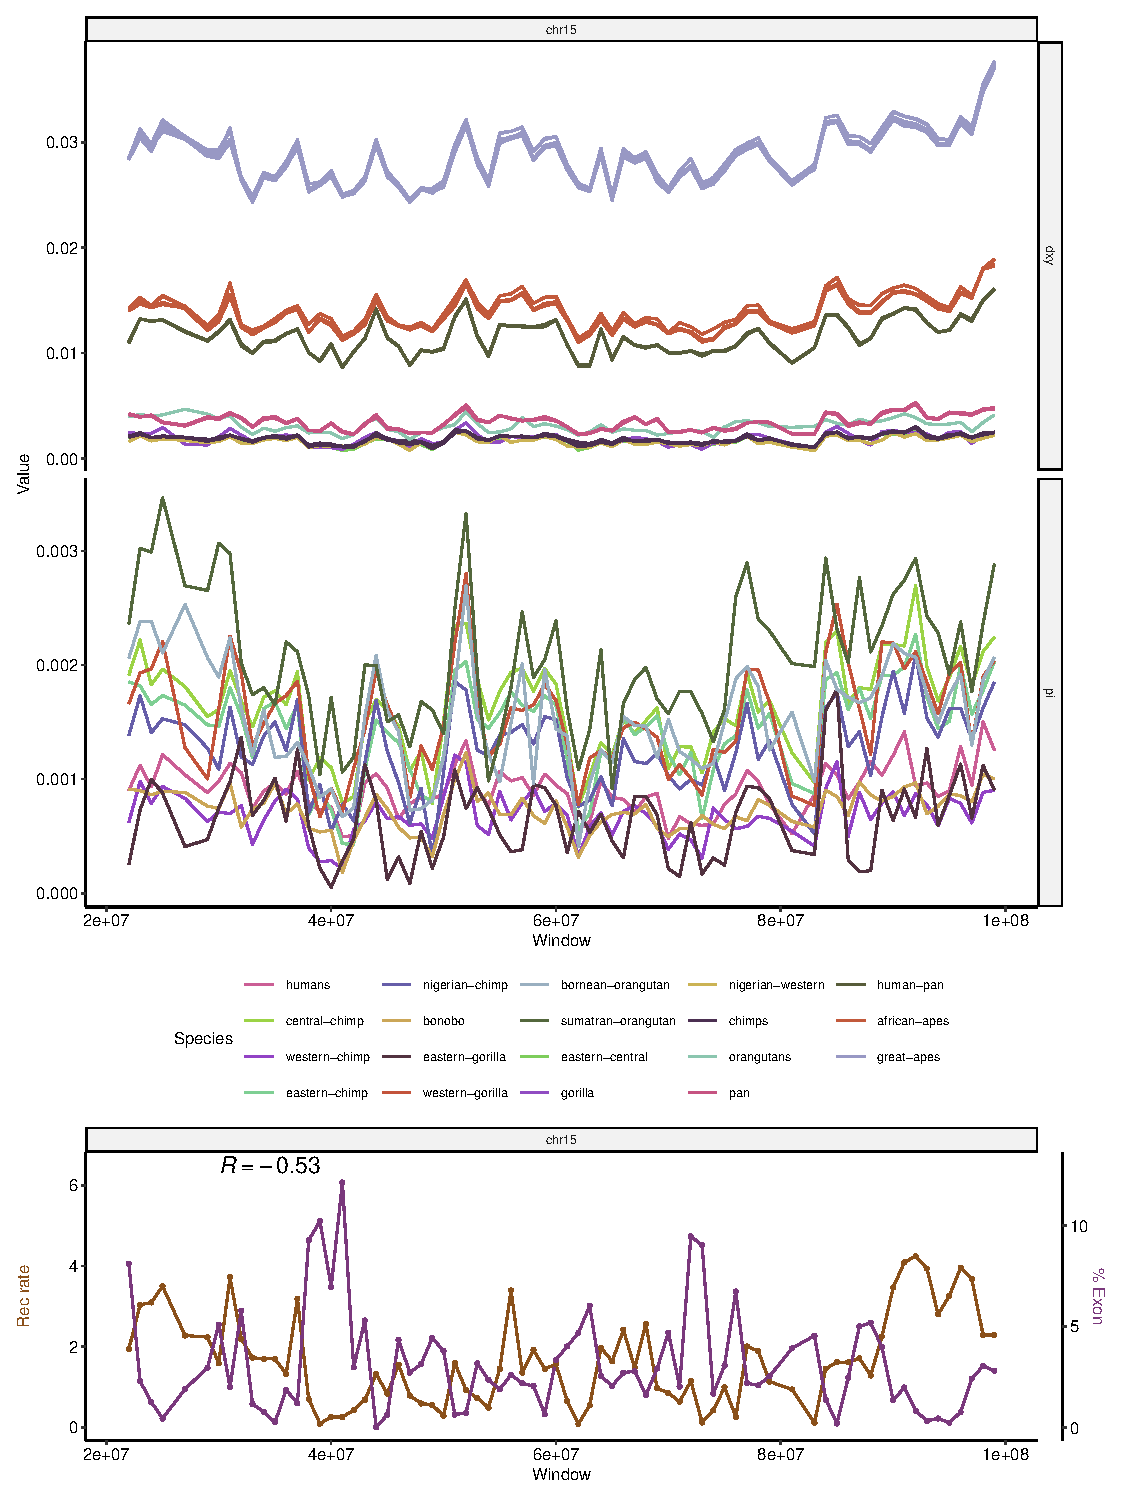
\includegraphics[width=\linewidth]{{figures/all-landscapes_chr15_win-size_1000000_merged-mask_True_state_all_curr_all_prop-acc_0.4.pdf}}
\centering
\caption{
Landscapes of diversity, divergence, exon density and recombination rate across chromosome 15.
See \lcref{fig:chr12_landscapes} for more details.
}
\label{fig:chr15_land}
\end{figure}

\begin{figure}[htp]
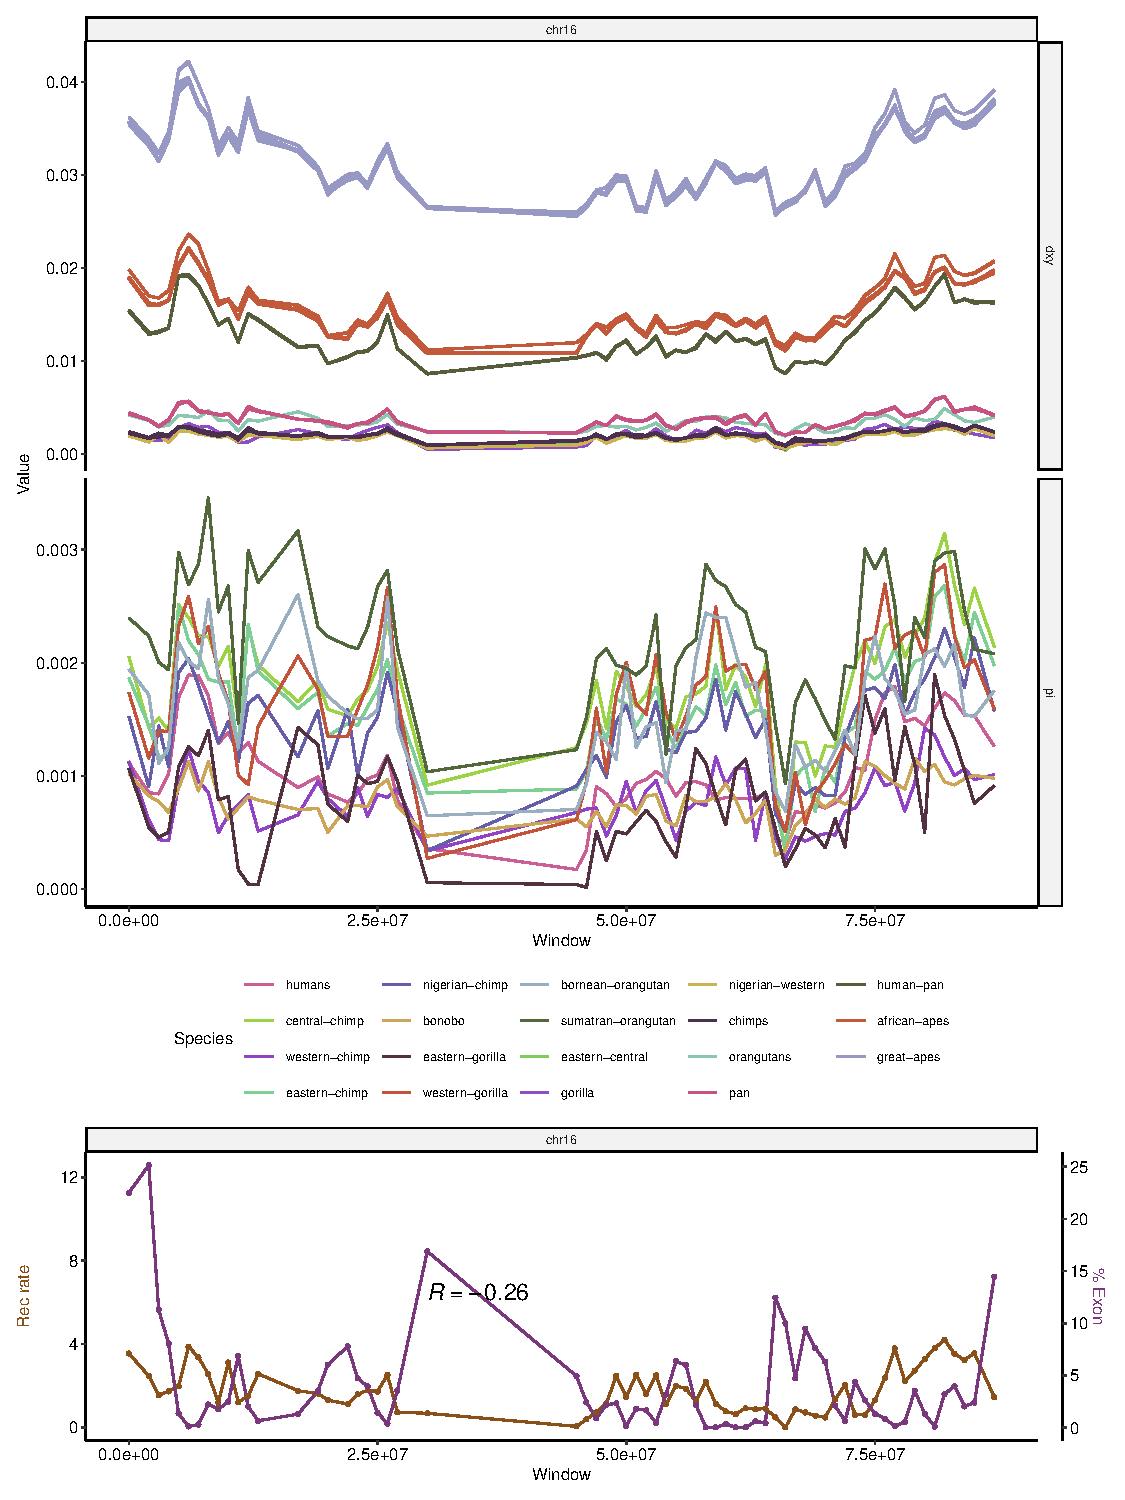
\includegraphics[width=\linewidth]{{figures/all-landscapes_chr16_win-size_1000000_merged-mask_True_state_all_curr_all_prop-acc_0.4.pdf}}
\centering
\caption{
Landscapes of diversity, divergence, exon density and recombination rate across chromosome 16.
See \lcref{fig:chr12_landscapes} for more details.
}
\label{fig:chr16_land}
\end{figure}

\begin{figure}[htp]
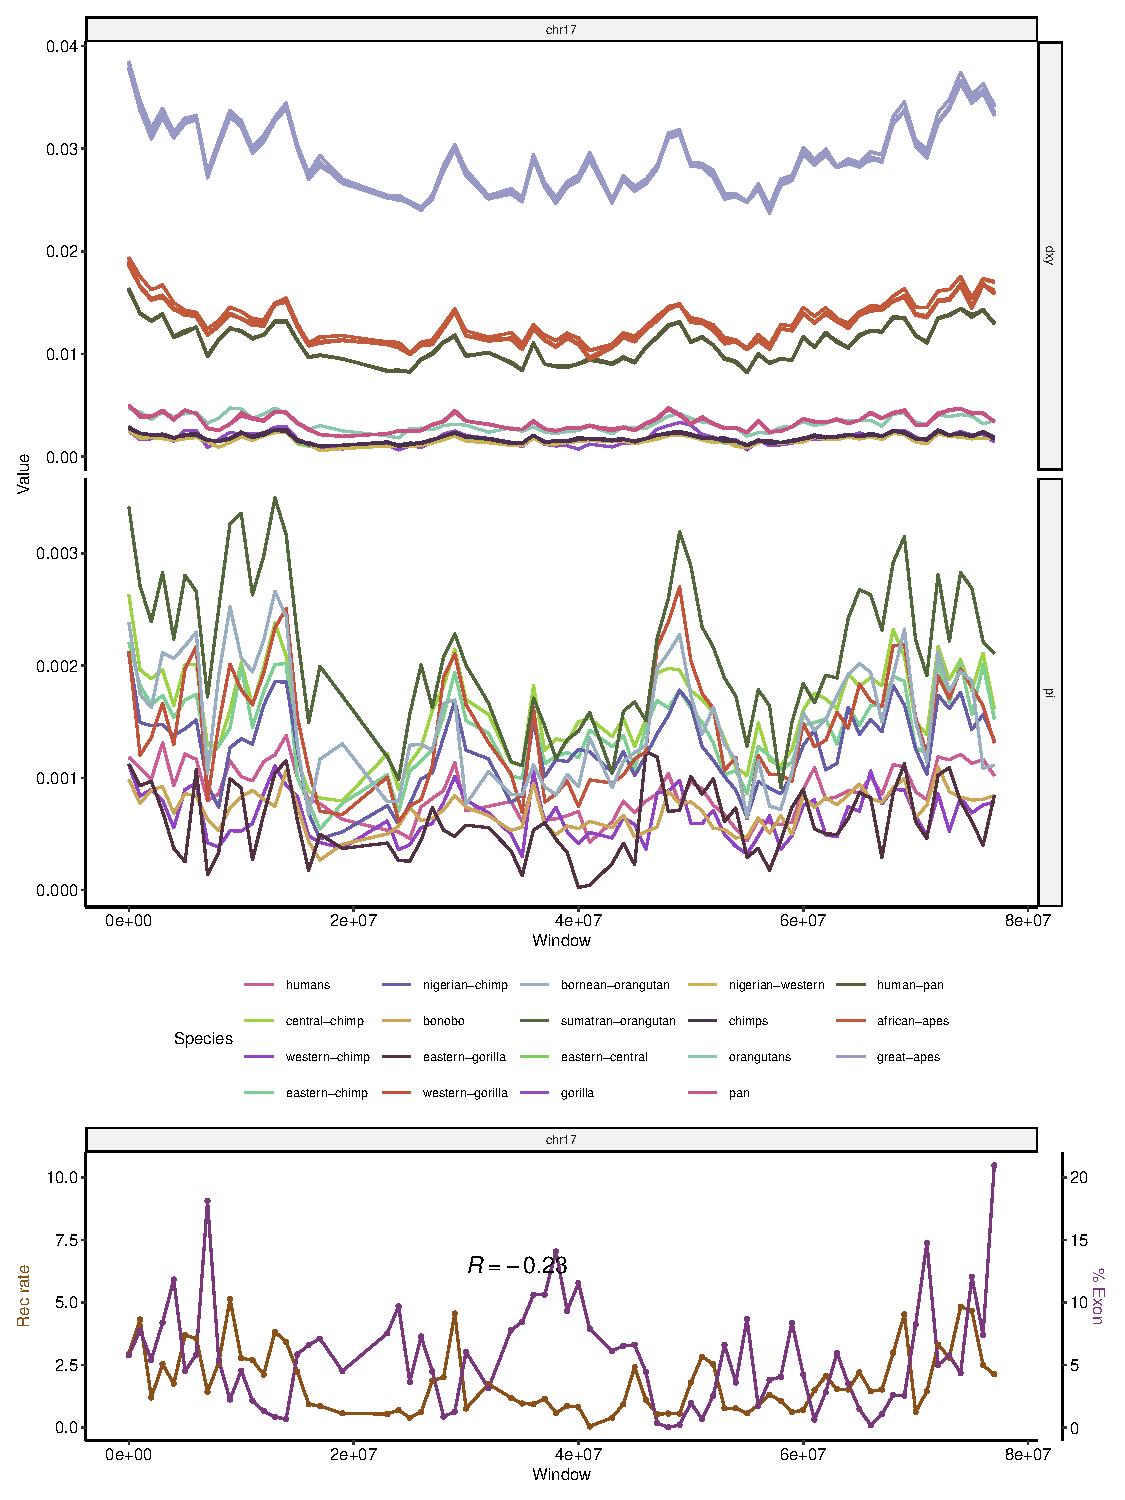
\includegraphics[width=\linewidth]{{figures/all-landscapes_chr17_win-size_1000000_merged-mask_True_state_all_curr_all_prop-acc_0.4.pdf}}
\centering
\caption{
Landscapes of diversity, divergence, exon density and recombination rate across chromosome 17.
See \lcref{fig:chr12_landscapes} for more details.
}
\label{fig:chr17_land}
\end{figure}

\begin{figure}[htp]
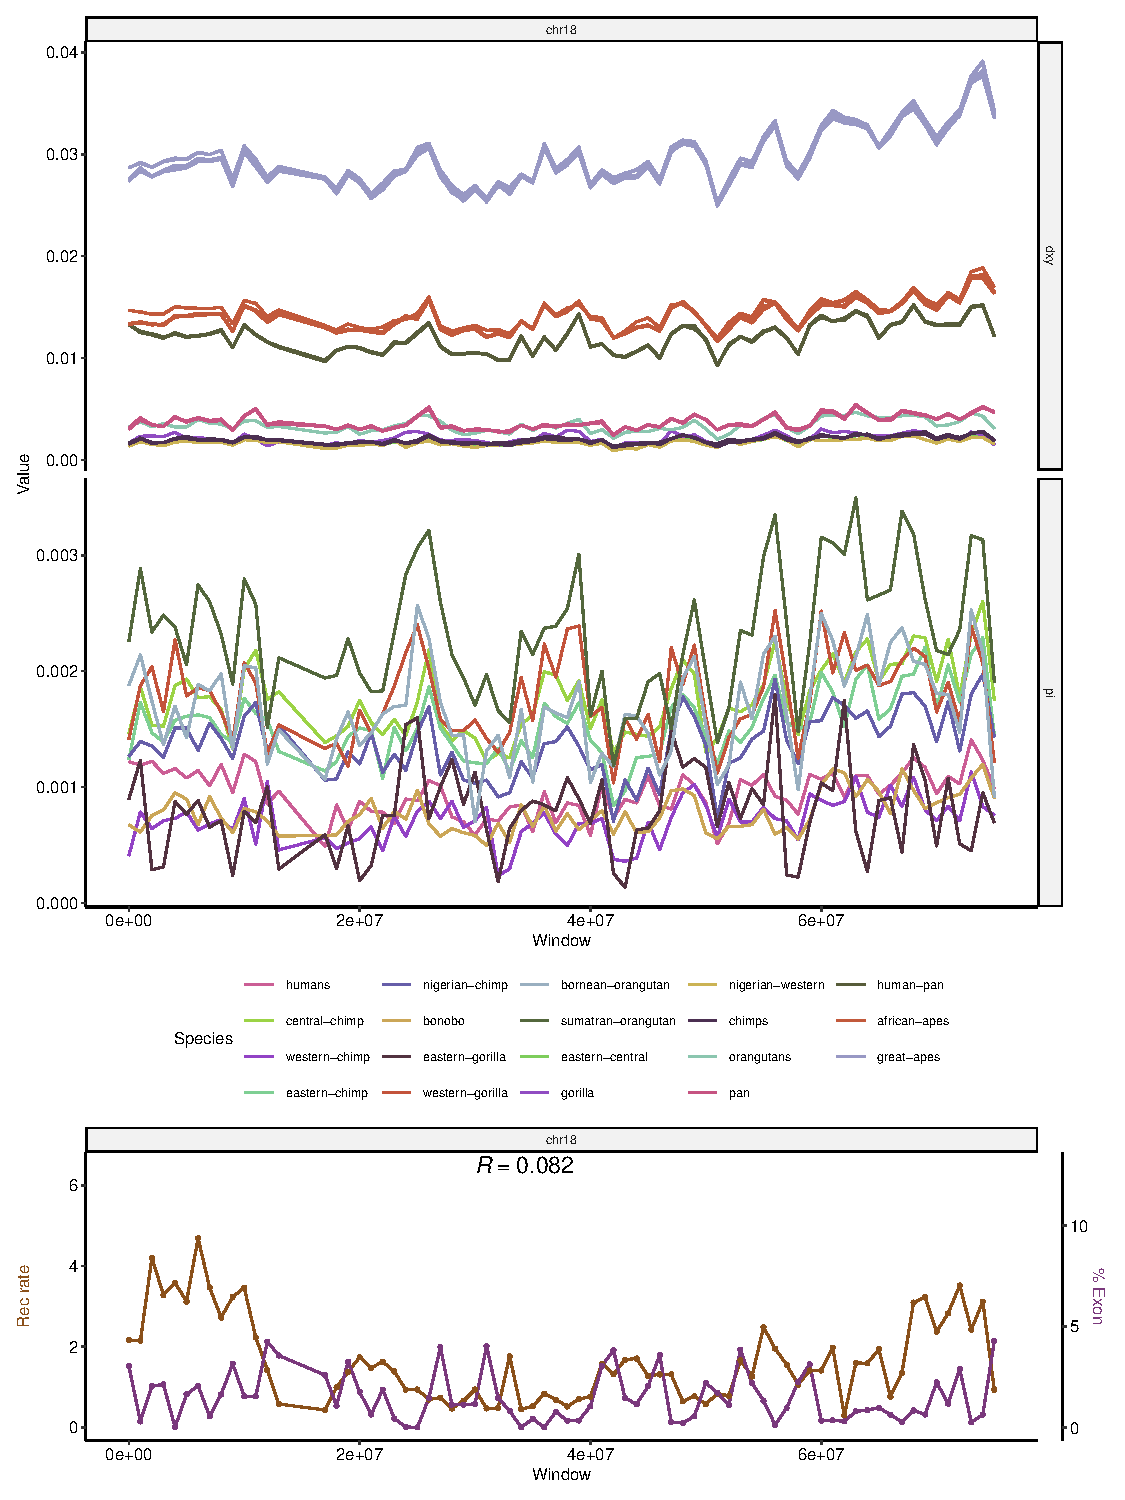
\includegraphics[width=\linewidth]{{figures/all-landscapes_chr18_win-size_1000000_merged-mask_True_state_all_curr_all_prop-acc_0.4.pdf}}
\centering
\caption{
Landscapes of diversity, divergence, exon density and recombination rate across chromosome 18.
See \lcref{fig:chr12_landscapes} for more details.
}
\label{fig:chr18_land}
\end{figure}

\begin{figure}[htp]
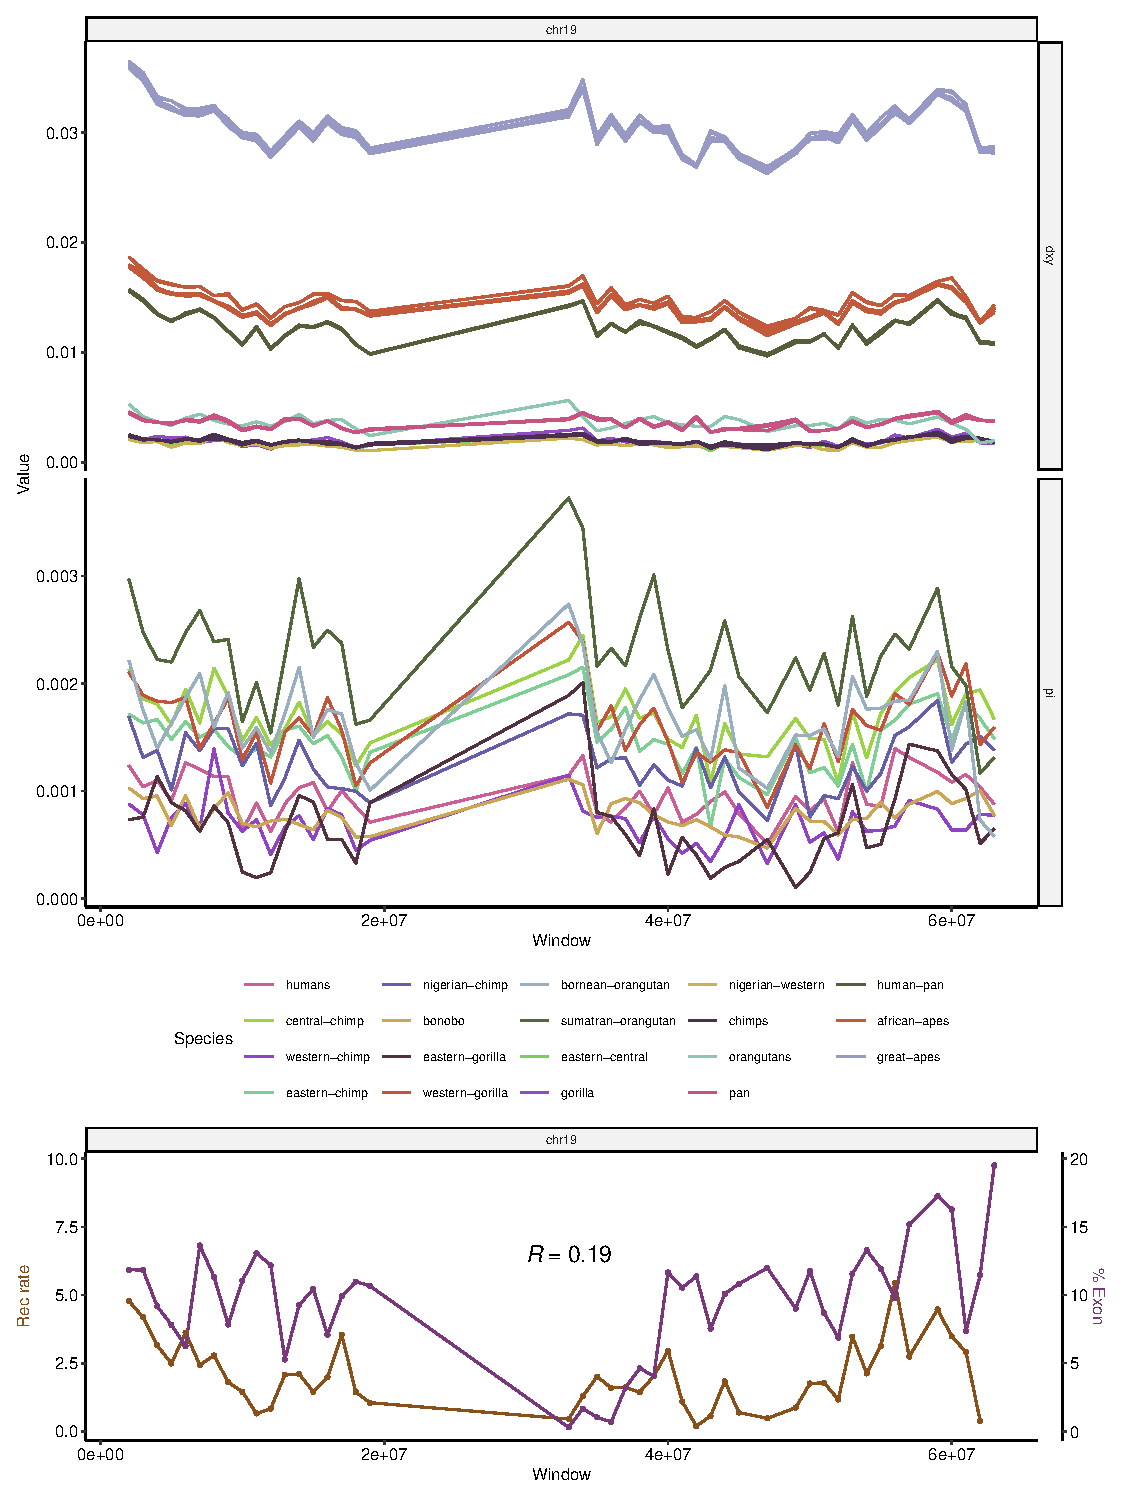
\includegraphics[width=\linewidth]{{figures/all-landscapes_chr19_win-size_1000000_merged-mask_True_state_all_curr_all_prop-acc_0.4.pdf}}
\centering
\caption{
Landscapes of diversity, divergence, exon density and recombination rate across chromosome 19.
See \lcref{fig:chr12_landscapes} for more details.
}
\label{fig:chr19_land}
\end{figure}

\begin{figure}[htp]
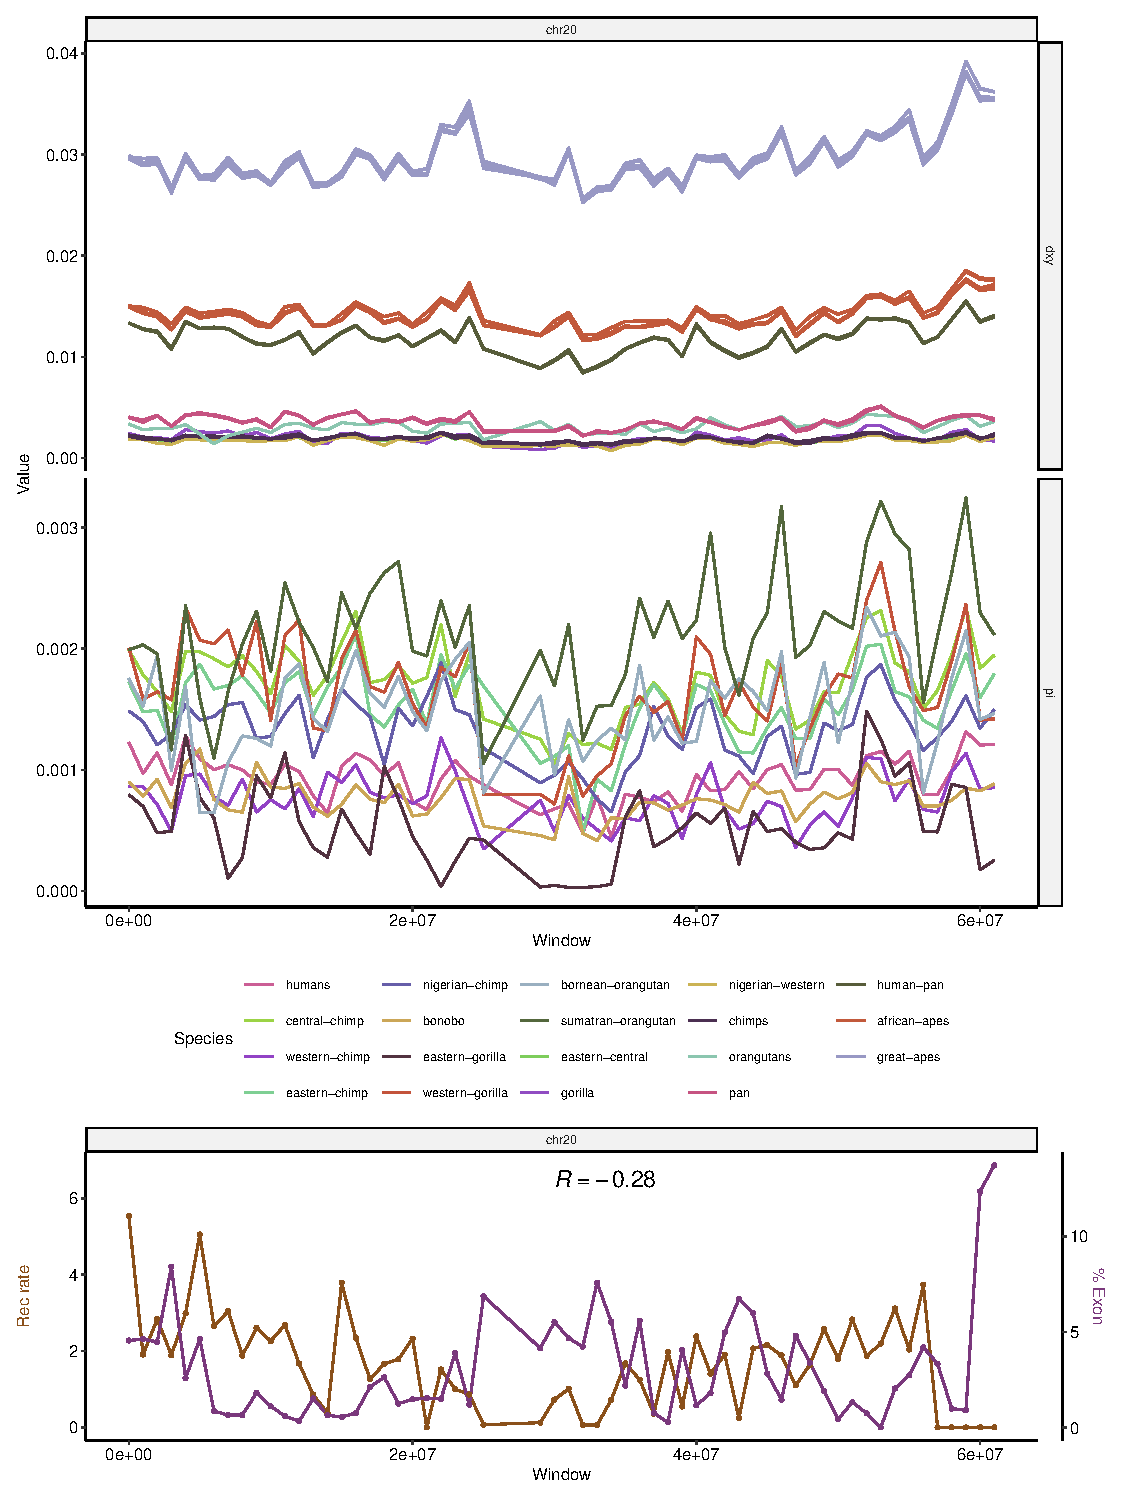
\includegraphics[width=\linewidth]{{figures/all-landscapes_chr20_win-size_1000000_merged-mask_True_state_all_curr_all_prop-acc_0.4.pdf}}
\centering
\caption{
Landscapes of diversity, divergence, exon density and recombination rate across chromosome 20.
See \lcref{fig:chr12_landscapes} for more details.
}
\label{fig:chr20_land}
\end{figure}

\begin{figure}[htp]
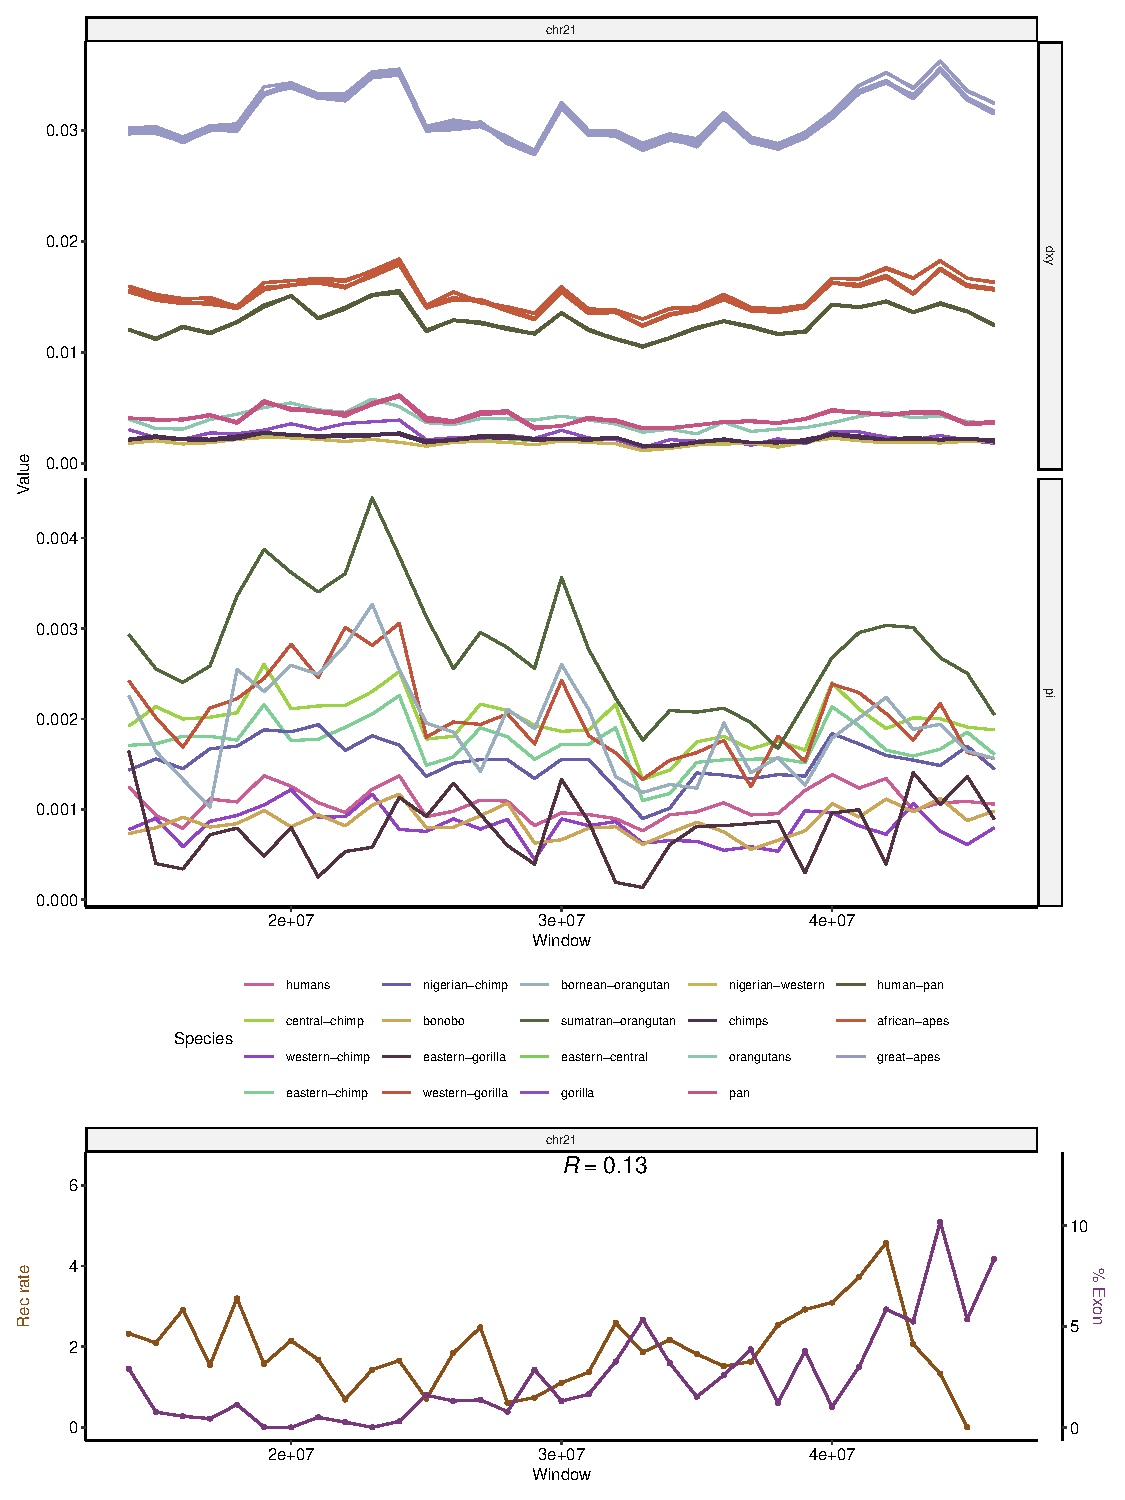
\includegraphics[width=\linewidth]{{figures/all-landscapes_chr21_win-size_1000000_merged-mask_True_state_all_curr_all_prop-acc_0.4.pdf}}
\centering
\caption{
Landscapes of diversity, divergence, exon density and recombination rate across chromosome 21.
See \lcref{fig:chr12_landscapes} for more details.
}
\label{fig:chr21_land}
\end{figure}

\begin{figure}[htp]
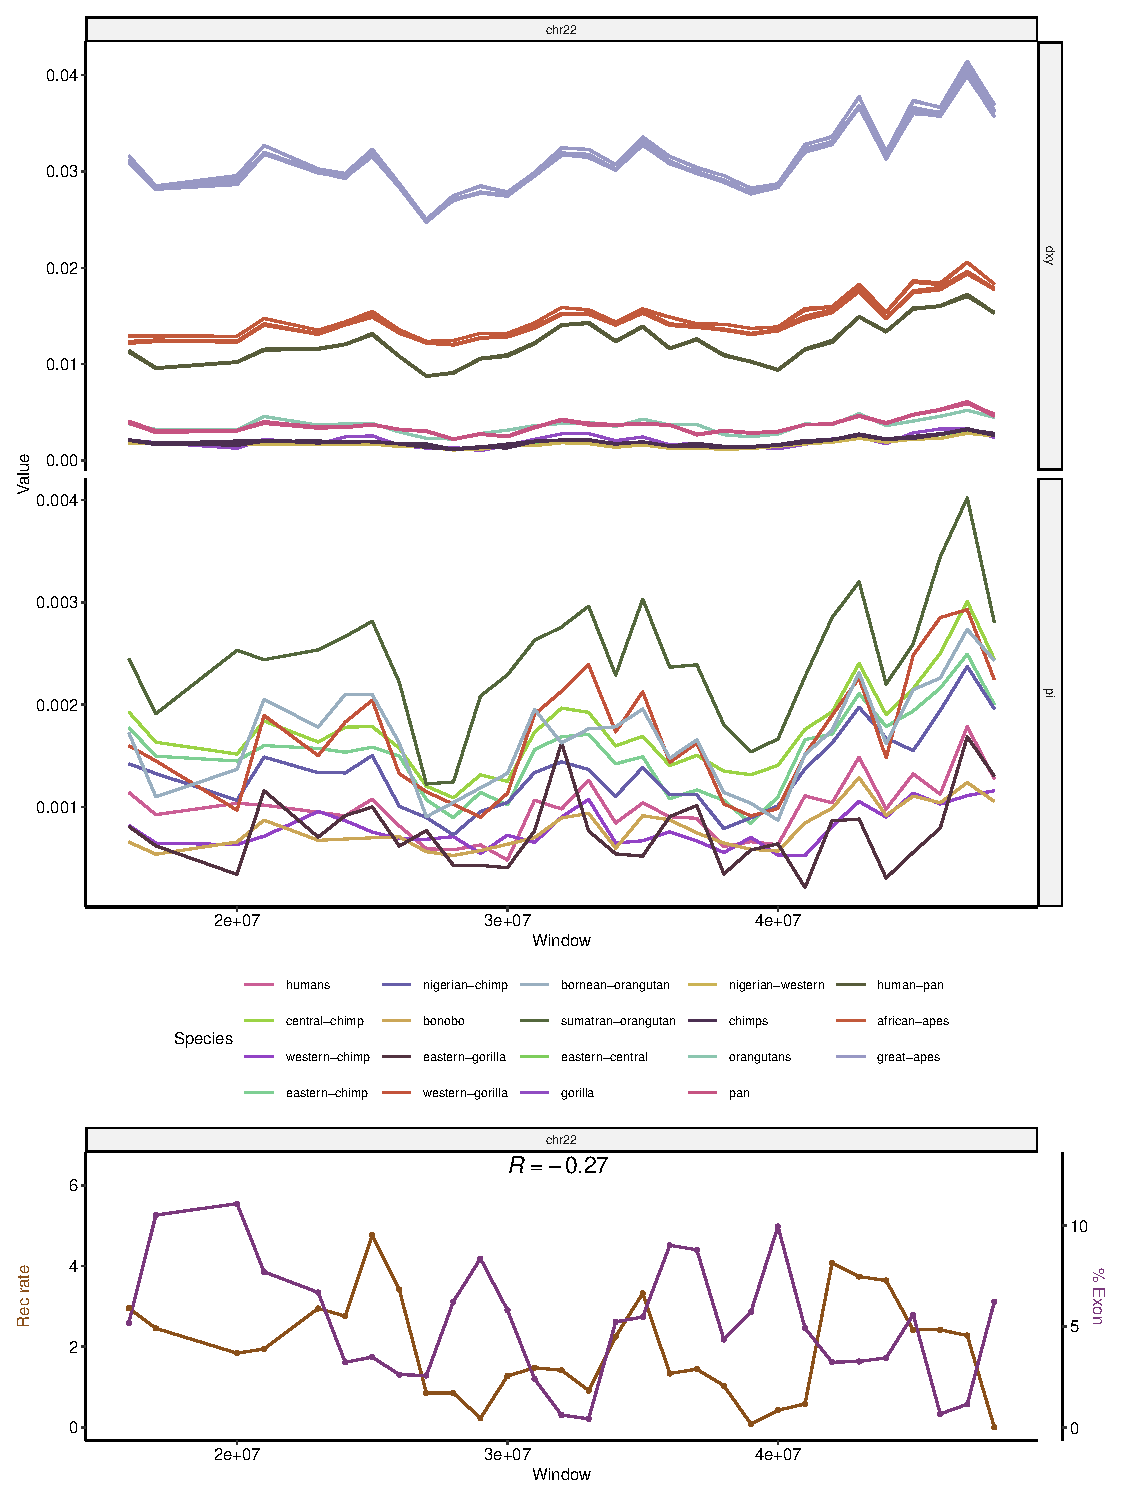
\includegraphics[width=\linewidth]{{figures/all-landscapes_chr22_win-size_1000000_merged-mask_True_state_all_curr_all_prop-acc_0.4.pdf}}
\centering
\caption{
Landscapes of diversity, divergence, exon density and recombination rate across chromosome 22.
See \lcref{fig:chr12_landscapes} for more details.
}
\label{fig:chr22_land}
\end{figure}

